%! Author = amatarazzo
%! Date = 10/03/24


\chapter{Introduction to Large Language Models}
\label{ch:introduction}


\section{Definition and Overview}
\label{sec:definition-and-overview}

In the contemporary landscape of artificial intelligence, Large Language Models (LLMs) stand out as monumental achievements, revolutionising natural language processing.
These models, characterised by their immense scale and complexity, have become pivotal in understanding and generating human-like text.
At their core, LLMs are designed to comprehend, learn, and generate coherent and contextually relevant language on an unparalleled scale.

Historically, the development of Language Models (LMs) has been rooted in the quest to understand and replicate human language, and four main stages can be identified:
\begin{enumerate}
	\item \textbf{Statistical Language Models:} {These models were developed to capture the statistical properties of language, such as word frequencies and co-occurrences, to predict the likelihood of a given sequence of words based on the Markov assumption, which states that the probability of a word depends only on the previous \textit{n} words.
		      If the context length \textit{n} is fixed, the model is called an \textit{n}-gram model.\\
		      However, these models are limited by the exponential number of transition probabilities to be estimated and the Markov assumption, which may not always hold true in the complexity of natural languages.
		      Language understanding often involves capturing dependencies over longer distances than the Markov assumption allows. Models considering broader contexts, such as recurrent neural networks (RNNs) and transformers, have been developed to address these long-range dependencies in language processing tasks.}
	\item \textbf{Neural Language Models:} {The advent of neural networks led to the development of language models that utilised neural architectures to capture language's complex patterns and dependencies.
		      These models, such as recurrent neural networks (RNNs) and long short-term memory (LSTM) networks, could capture long-range dependencies and contextual information, enabling them to generate coherent and contextually relevant text.
		      \textcite{bengio2003neural} introduced the concept of \textit{distributed representation} of words and built the word prediction function of the distributed word vectors.
		      Later, word2vec~\cite{mikolov2013distributed, mikolov2013efficient} introduced the word2vec model, a shallow, two-layer neural network trained to reconstruct the linguistic contexts of words.
		      These models were a significant leap forward in the development of language models, representing a shift from word sequencing to learning representation.}
	\item \textbf{Pre-trained language models (PLM):} {The development of pre-trained language models (PLMs) marked a significant milestone in the evolution of language models.
		      These models were trained on large data corpora in an unsupervised or self-supervised manner before being fine-tuned on specific tasks. The idea is to pre-train a model on a diverse data set and then transfer its knowledge to a narrower task by fine-tuning it on a smaller, task-specific dataset.
		      ELMo~\footnote{Embeddings from Language Models}~\cite{peters2018deep} was one of the first PLMs which used a bidirectional LSTM to generate word embeddings instead of learning fixed word representations.
		      \textcite{devlin2019bert} introduced BERT (Bidirectional Encoder Representations from Transformers), a transformer-based model pre-trained on a large corpus of text and then fine-tuned it on specific tasks.
		      BERT was a significant advancement in natural language processing, as it demonstrated the potential of pre-trained language models to achieve state-of-the-art performance on a wide range of tasks.
		      These studies introduced the \textit{"pre-training and fine-tuning"} paradigm, which has become a standard practice in the development of language models and inspired a significant number of models, such as GPT-2~\cite{radford2019language}), GPT-3 (\textcite{brown2020language}), T5 (\textcite{raffel2023exploring}, and many others.
	      }
	\item \textbf{Large Language Models (LLM):} {The emergence of large language models, characterised by their immense scale and complexity, has redefined the capabilities of language processing systems.
		      Studies find that language models' performance improves as the number of parameters (e.g., model size) or data size increases, a phenomenon known as the scaling law in large language models.
		      Many LLMs are built on the transformer architecture, designed to capture long-range dependencies and contextual information in language.
		      The transformer architecture has become the foundation for many state-of-the-art language models. Unlike earlier models that were unidirectional (e.g., traditional RNNs), LLMs, especially those based on transformers, are bidirectional. They consider the context of preceding and following words, enhancing their language understanding.
		      LLMs find applications across various domains, including but not limited to:
		      \begin{itemize}
			      \item \textbf{Text Generation:} Producing coherent and contextually relevant text.
			      \item \textbf{Question Answering:} Answering questions based on provided context.
			      \item \textbf{Language Translation:} Translating text from one language to another.
			      \item \textbf{Summarization:} Creating concise summaries of longer texts.
			      \item \textbf{Sentiment Analysis:} Determining the sentiment expressed in a text.
		      \end{itemize}
		      These large-sized PLMs have been shown to outperform their smaller (e.g., 330M-parameters vs 1.5B-parameters) and show surprising capabilities \footnote{Note that a LLM is not necessarily more capable than a small PLM, and emergent abilities may not occur in some LLMs.}, also called emergent abilities by \textcite{wei2022emergent}.
		      \begin{displayquote}
			      Emergence is when quantitative changes in a system result in qualitative changes in behavior~\cite{anderson1972more}.
		      \end{displayquote}
		      These emergent abilities include but are not limited to, the ability to perform tasks for which they were not explicitly trained, such as translation, summarisation, and question-answering, and to generalise to new tasks and domains, such as zero-shot learning \footnote{It refers to a machine learning scenario where a model makes predictions or performs tasks for classes or examples it has never seen during training}, few-shot learning \footnote{It involves training a model with a minimal number of examples per class, usually much fewer than what traditional machine learning models require}, and even one-shot\footnote{It is a specific case of few-shot learning where the model is trained with only one example per class} learning\footnote{A shot is an example or demonstration of what type of prompt and response you expect from a large language model. This term originates from training computer vision models on photographs, where one shot was one example or instance that the model used to classify an image \cite{feifei2006onedatacoltut}.}.
		      Three typical examples of emergent abilities are:
		      \begin{enumerate}
			      \item \textbf{In-context learning:} {this ability has been formally observed in GPT-3, which is provided with a natural language instruction or task demonstrations; it can generate the expected output for test instances by completing the word sequence of the input text. Importantly, this can be achieved without requiring additional training or gradient updates \footnote{Recent study shows that in-context learning implicitly performs meta optimisation through the attention mechanism~\cite {dai2022why}}.
				            \begin{quote}
					            \textbf{Language Translation:} \\
					            \textit{Input:} {\enquote{Translate the following English text to French: `The quick brown fox jumps over the lazy dog.'}} \\
					            \textit{Output:} {\enquote{Le renard brun rapide saute par-dessus le chien paresseux.}}\\
					            \textbf{Arithmetic Tasks:} \\
					            \textit{Input:} {\enquote{What is the sum of 42 and 63?}} \\
					            \textit{Output:} {\enquote{The sum of 42 and 63 is 105.}}
				            \end{quote}
			            }
			      \item \textbf{Instruction following:}{
				            Through the process called instruction tuning -- that we will see more in-depth in Section  \ref{subsec:instruction-tuning} -- LLMs exhibit strong performance on unseen tasks described through natural language instructions \cite{sanhetal2022multitask, ouyang2022training, wei2022fine}.
				            This approach involves fine-tuning the model using diverse multitask datasets, each accompanied by detailed natural language descriptions. The result is an LLM that effectively interprets and follows instructions for new and unseen tasks without relying on explicit examples.
				            Experiments detailed in \textcite{wei2022fine} demonstrate that LaMDA-PT, fine-tuned with instructions, begins to outperform its untuned counterpart significantly when the model size reaches 68 billion parameters. However, this performance gain is not observed for 8 billion or smaller model sizes. Furthermore, \textcite{chung2022scaling} highlights that a model size of at least 62 billion parameters is necessary for PaLM to excel across various tasks in evaluation benchmarks like MMLU, BBH, TyDiQA, and MGSM. Nevertheless, it is noted that certain specific tasks, such as MMLU, might suffice with much smaller model size, emphasising the nuanced relationship between model size and task performance.
			            }
			      \item \textbf{Step-by-step reasoning:} { For small LMs, it is usually difficult to solve complex tasks that involve multiple reasoning steps (e.g., mathematical word problems).
				            In contrast, the chain-of-thought (CoT) prompting strategy \cite{wei2022chain} empowers Large Language Models (LLMs) to surmount these challenges. By leveraging the CoT prompting mechanism, which involves intermediate reasoning steps to derive the final solution, LLMs exhibit proficiency in tasks requiring intricate cognitive processes. This capability is speculated to be honed through training on code by \textcite{wei2022chain}. Empirical findings in \textcite{wei2022chain} demonstrate that the employment of CoT prompting yields performance gains, particularly on arithmetic reasoning benchmarks, when applied to variants of models like PaLM and LaMDA, especially with a model size surpassing 60B. The advantages of CoT prompting become more pronounced as the model size exceeds 100B. Furthermore, the effectiveness of CoT prompting exhibits variability across different tasks, with performance improvement observed in the order of GSM8k~\textgreater~MAWPS~\textgreater~SWAMP for PaLM~\cite{wei2022chain}.
			            }
		      \end{enumerate}
	      }
\end{enumerate}
The advent of LLMs has led to a paradigm shift in the field of natural language processing, with applications ranging from machine translation to text summarisation and from question-answering systems to language generation.
The development of LLMs has been driven by the exponential growth of data and computational resources, which has enabled the training of models with billions of parameters.
The scale of these models has enabled them to capture complex patterns in language and generate coherent and contextually relevant text.

The potential of LLMs is vast, and their impact on natural language processing is profound.
The advent of ChatGPT~\cite{adiwardana2020towards} and GPT-4~\cite{openai2024gpt4} has further expanded the capabilities of LLMs, leading to the rethinking of the possibilities of artificial general intelligence (AGI).

Regarding NLP, LLMs can serve somewhat as general-purpose language task solvers.
In the IR field, LLMs can be used to improve the performance of information retrieval systems through AI chatbots (i.e., ChatGPT) and New Bing \footnote{https://www.microsoft.com/it-it/bing?form=MA13FV}.
In the CV field, LLMs can be used to improve the performance of computer vision systems through multimodal models \footnote{
	Models are designed to process and understand information from multiple modalities or sources (e.g., text, image, audio, video).
	Multimodal models aim to handle and integrate data from two or more modalities.
} (i.e., CLIP\footnote{Contrastive Language–Image Pre-training}~\cite{radford2021learning} and DALL-E~\cite{ramesh2021zero}).

This work will mainly focus on model sizes larger than 10B parameters to explore their capabilities, limitations, and potential applications.
We will delve into the emergent abilities of LLMs, such as in-context learning, instruction following, and step-by-step reasoning, and how these abilities can be leveraged to solve complex tasks in Chapter~\ref{ch:utilization}.
The study will investigate and compare the abilities of different LLMs, focusing on the impact of various parameters on their performance.


\section{Scaling Law}
\label{sec:scaling-law-in-large-language-models}

The Scaling Law in LLMs constitutes a fundamental principle underlining their development and performance.
At its essence, the scaling law posits that as language models increase in size, their capabilities and performance on linguistic tasks exhibit disproportionately positive growth.
This concept has become a guiding force in pushing the boundaries of language processing and understanding.

As LLMs scale up in terms of parameters, encompassing tens or hundreds of billions, or even trillions, they demonstrate an unprecedented ability to generalise from diverse datasets and generate contextually coherent text.
The essence of the scaling law lies in the direct correlation between the size of a language model and the number of parameters it encompasses.
Parameters are the internal variables the model learns during training, representing the connections and weights defining its understanding of language.
As the number of parameters increases, so does the model's capacity to encapsulate complex linguistic structures.

One primary outcome of adhering to the scaling law is the substantial improvement in performance across a spectrum of language-related tasks.
From language generation to sentiment analysis, question-answering, and summarization, larger models consistently outperform their smaller counterparts.
The increased capacity for learning intricate language features enables LLMs to excel in understanding and producing more human-like text.

When writing, most of the LLMs are based on the transformer architecture, where multi-headed self-attention layers are stacked in a very deep neural network.
We'll dive deep into the transformer architecture in Section~\ref{subsec:transformer-architecture}, but for now, we can say that self-attention is a mechanism that allows a model to weigh different parts of the input sequence differently, capturing dependencies between words.
The multi-headed self-attention mechanism lets the model capture different dependencies and relationships between words, enhancing language understanding.
The idea is that different attention heads can focus on different aspects or relationships within the data, allowing the model to capture more nuanced patterns.
Multiple layers of these multi-headed self-attention mechanisms are stacked in a very deep neural network.
Each layer in the stack processes the previous layer's output, learning hierarchical representations of the input data and capturing increasingly complex relationships and abstractions. \\
Two representative scaling laws for Transformer-based LLMs are the following~\cite{kaplan2020scaling, hoffmann2022training}:
\begin{enumerate}
	\item \textbf{KM scaling law:} {named in this way in \textcite{survey} and proposed by the OpenAI team in \textcite{kaplan2020scaling}. Given model size $M$, dataset size $D$, amount of training compute $C$, and a compute budget $c$, the KM scaling law states that the performance of a language model scales as per the following three formulas:

		      \begin{equation}
			      \begin{aligned}
				      L(N) & =(\frac{N_c}{N})^{\alpha_N}, \alpha_N \approx 0.076, N_c \approx 8.8 \times 10^{13} \\
				      L(D) & =(\frac{D_c}{D})^{\alpha_D}, \alpha_D \approx 0.095, D_c \approx 5.4 \times 10^{13} \\
				      L(C) & =(\frac{C_c}{C})^{\alpha_C}, \alpha_C \approx 0.050, C_c \approx 3.1 \times 10^8
			      \end{aligned}
			      \label{eq:km-scaling-law}
		      \end{equation}

		      \noindent where $L(N)$, $L(D)$, and $L(C)$ denote the cross-entropy loss of the model, the dataset, and the amount of training computed, respectively.
		      The three laws were formulated by analysing the model's performance across a range of data sizes (from 22M to 23B tokens), model sizes (from 768M to 1.5B non-embedding parameters), and training compute, with certain assumptions (e.g., ensuring that the other two factors do not constrain the analysis of one factor).
		      The findings demonstrated a robust interdependence among the three factors influencing model performance.
	      }
	\item \textbf{Chinchilla scaling law:} {An alternative form of the scaling law has been proposed by the Google DeepMind team in \textcite{hoffmann2022training} experimenting with an extensive range of model size (70M to 16B) and data sizes (5B to 500B tokens).
		      The Chinchilla scaling law posits that the performance of a language model scales as per the following formula:

		      \begin{equation}
			      L(N,D) = E + \frac{A}{N^\alpha} + \frac{B}{D^\beta},
			      \label{eq:chinchilla-scaling-law}
		      \end{equation}
		      \noindent where $E=1.69, A=406.4,B = 410.7, \alpha = 0.34, \beta = 0.28$

		      Authors showed that optimal allocation of compute budget to model size and data size can be derived as follows \footnote{under the constraint \(C \approx 6ND\)}:

		      \begin{center}
			      \begin{equation}
				      N_{opt}(C) = G(\frac{C}{6})^a, D_{opt}(C) = G^{-1}(\frac{C}{6})^b, \label{eq:optimal-allocations}
			      \end{equation}
		      \end{center}

		      \noindent where $a=\frac{\alpha}{\alpha+\beta}, b=\frac{\beta}{\alpha+\beta}$ and G is a scaling coefficient.
		      The KM scaling law favours a more significant budget allocation in model size than the data size. In contrast, the Chinchilla scaling law argues that the two sizes should be increased in equal scales \cite{hoffmann2022training} (i.e., having similar values for a and b in \eqref{eq:optimal-allocations}).
	      }
\end{enumerate}

Scaling boosts performance and addresses inherent limitations in smaller language models.
Larger models excel in managing long-range dependencies, comprehending ambiguous language constructs, and displaying a nuanced understanding of context---capabilities that smaller models frequently find challenging.
The eliciting of emergent abilities, such as Chain-of-Thought prompting and in-context learning, have shown a phase change in the first Scaling Law, where the performance increases linearly as the model size increases exponentially (Figure~\ref{fig:scaling-phase}).
Emergency is still a debated topic, where some argue that emergency is dependent on the metrics used to evaluate the model's performance\cite{schaeffer2023emergentabilitieslargelanguage}, \footnote{Choosing a different metric it's possible to show that increasing the model size, leads to an improvement in correct sequences prediction in addition problems. Looking at this metrics, the add ability is not emergent, but gradual and predictable.}, while others still think that even when you have one-step predictions or use continuous metrics, you still have discontinuities, and as the model size increases, the performance increases in a jump-like manner.

At its core, the scaling law is a guiding principle in the development of LLMs, directing the allocation of resources and the design of models to maximise performance and capabilities.

\begin{figure}[h!]
	\centering
	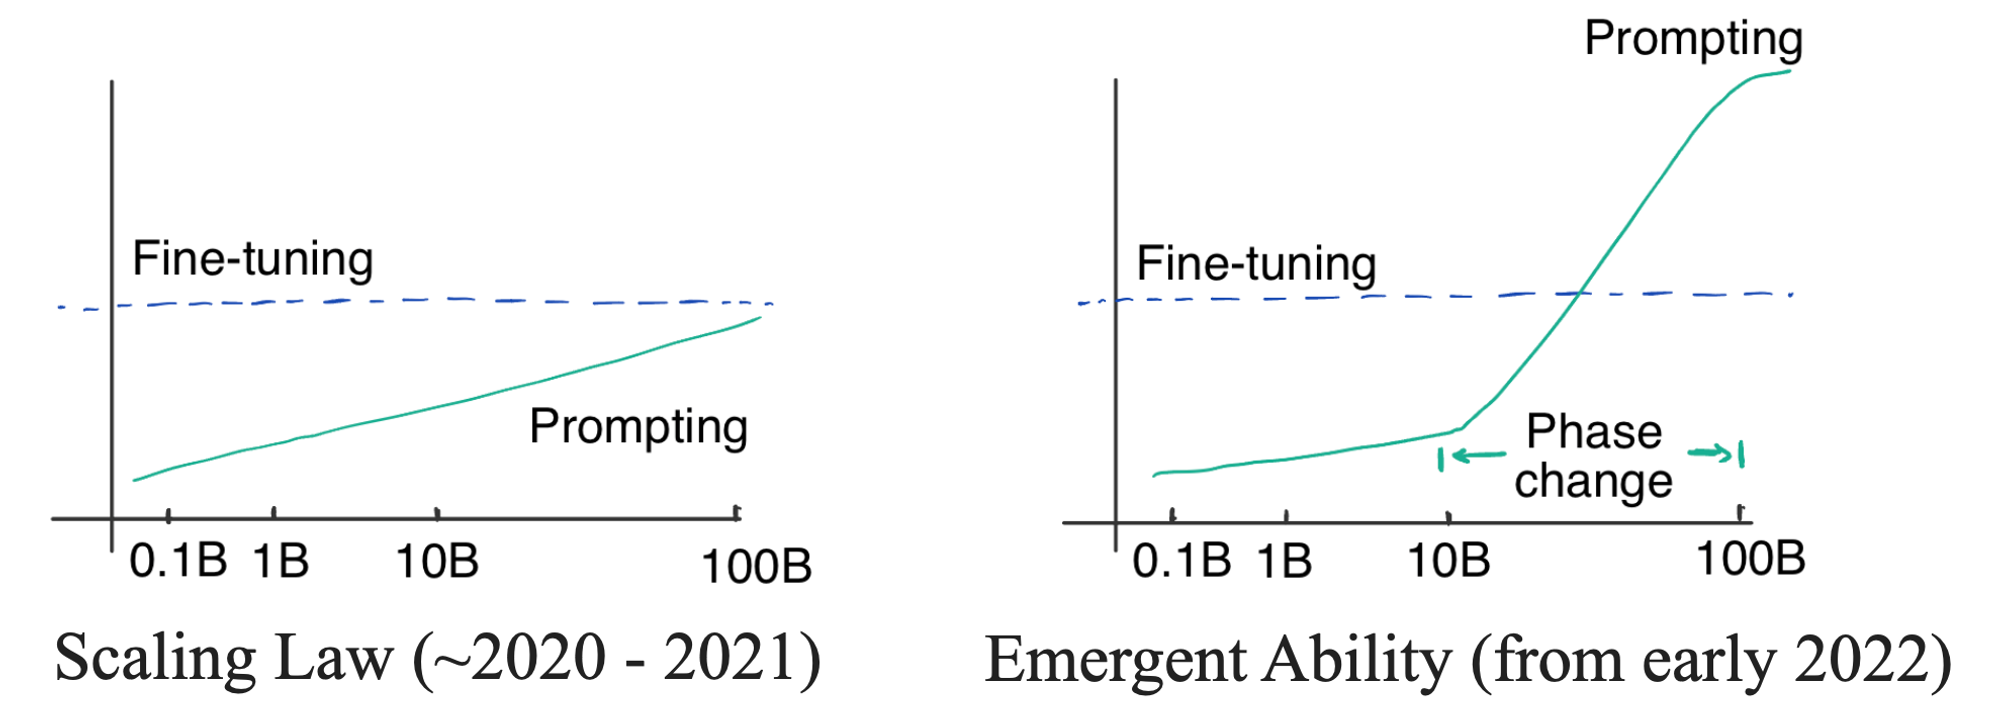
\includegraphics[width=0.7\textwidth]{scaling-phase}
	\caption{Left: scaling law. Model performance increases linearly as the model size increases exponentially. Right: emergent abilities show a phase change at a certain scale where the performance suddenly increases. Source: \textcite{yaofu2023emergent}.}
	\label{fig:scaling-phase}
\end{figure}

Despite propelling the field of LLMs to new heights, the scaling law comes with computational challenges.
Training huge models requires significant computational resources, encompassing processing power and memory.
The computational budget is an upper bound limit, demanding innovations in hardware and distributed training techniques to exploit the potential of scaled-up language models fully.

\section{Prominent Model Families}
\label{sec:promiment-model-families}

The development of Large Language Models (LLMs) has been driven by the emergence of prominent model families, each characterised by its unique architecture and capabilities.
These model families have played a pivotal role in shaping the landscape of language processing and understanding and have been instrumental in pushing the boundaries of LLMs.

Some of the most prominent large language models (having a size larger than 10B) are depicted in Figure~\ref{fig:llm-evolution}.

\begin{figure}[h!]
	\centering
	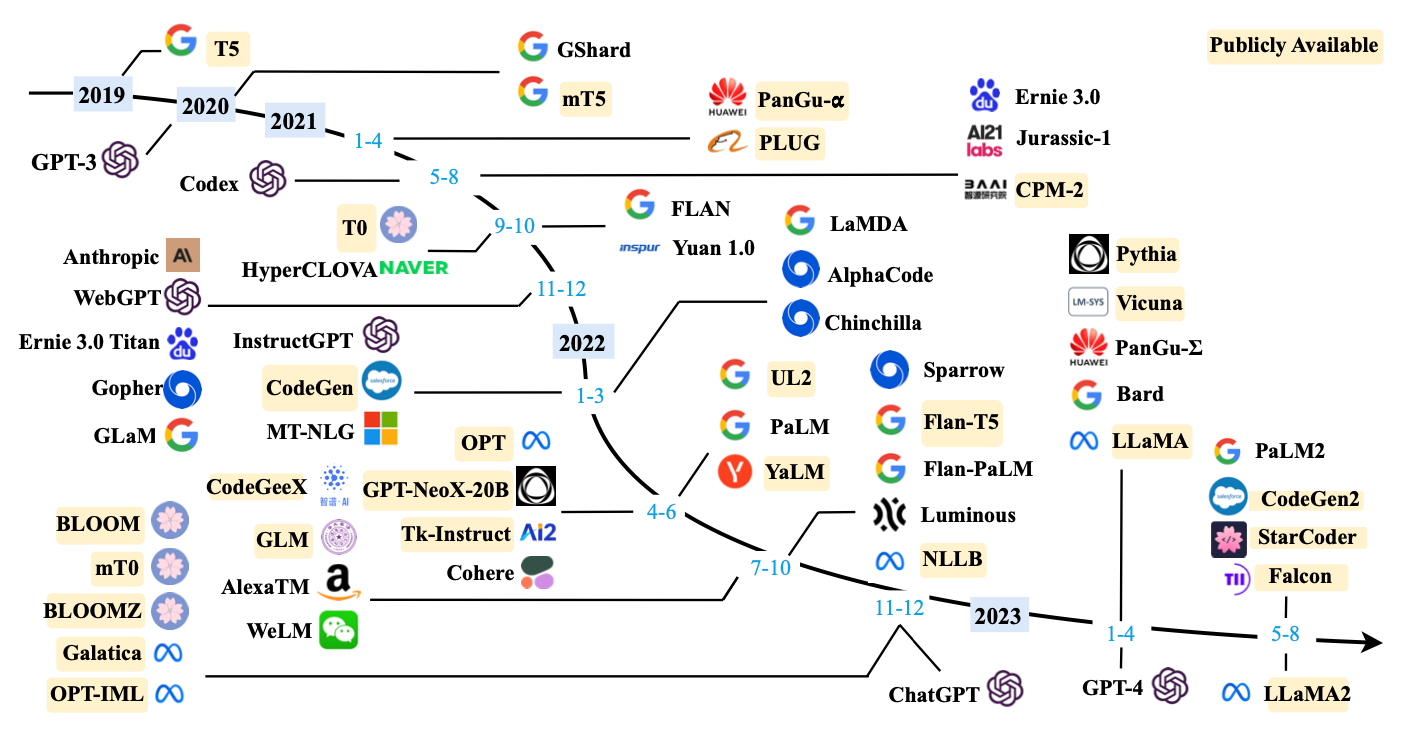
\includegraphics[width=\textwidth]{public_llm}
	\caption{A diagram showing the evolution of publicly available LLMs. Source: \textcite{survey}.}
	\label{fig:llm-evolution}
\end{figure}

\subsection{BERT}
\label{subsec:bert}

Introduced by Google in 2018, BERT~\cite{devlin2019bert} marked a significant evolution in LLMs by focusing on bidirectional context in text processing.
BERT's model architecture is a multi-layer bidirectional Transformer encoder based on the original transformer architecture introduced by \textcite{vaswani2023attention}.
Unlike its predecessors, BERT analyses text in both directions (left-to-right and right-to-left), providing a more nuanced understanding of language context.
This bi-directionality enables BERT to achieve state-of-the-art results in various NLP tasks, such as question answering, named entity recognition, and sentiment analysis.
BERT's architecture and training methodology have influenced numerous subsequent models and research initiatives~\cite{devlin2019bert}.

\begin{figure}[h!]
	\centering
	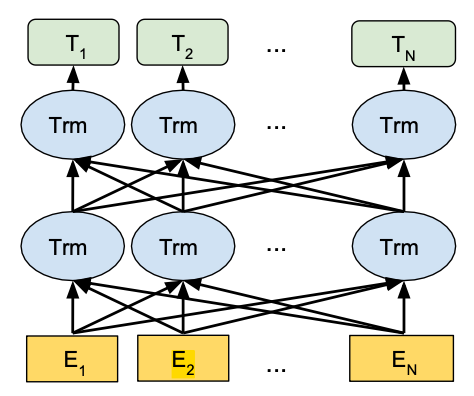
\includegraphics[width=0.5\textwidth]{bert}
	\caption{BERT Architecture: The bottom layer contains the embedding representations \(E_1, E_2, \ldots E_N\), which encode input tokens and serve as the input to the transformer layers (Trm).
		Each transformer bidirectionally processes the input embeddings, and the final output is used for downstream tasks. Source: \textcite{devlin2019bert}.}
	\label{fig:bert-arch}
\end{figure}

Even BERT is built on the transformer architecture~\cite{vaswani2023attention}, which relies heavily on attention mechanisms to understand the context of words in a sentence.
The innovation in BERT is its bidirectional nature and the use of a mechanism called the Masked Language Model (MLM). In MLM, some percentage of the input tokens are randomly masked, and the objective is to predict these masked tokens based on their context, leveraging information from both sides of the sequence.
BERT also incorporates a next-sentence prediction (NSP) task that helps the model learn relationships between sentences, further enhancing its understanding of context.

BERT's bidirectional context understanding significantly improves its performance on various NLP tasks, including sentiment analysis, question answering, and named entity recognition.
By pre-training on a large corpus of text and then fine-tuning on specific tasks, BERT can adapt to various domains with relatively little task-specific data, demonstrating impressive transfer learning capabilities.
Its architecture has set a new standard in the field, inspiring many subsequent models that build on or modify its foundational structure.

Despite its strengths, BERT is not without limitations.
The model's size and complexity require substantial computational resources for training, which can be a barrier for some organisations or researchers.
BERT's focus on context from surrounding text does not inherently solve all challenges in language understanding, particularly concerning ambiguity, nuance, or the subtleties of human language.
The model can sometimes struggle with tasks requiring extensive world knowledge or reasoning beyond the scope of its training data.

While BERT itself does not exhibit emergent abilities in the same way that scaling up GPT models does, its architecture has enabled new approaches to handling context and language understanding that were not feasible with prior models.
Subsequent iterations and variations of BERT, like RoBERTa\footnote{Robustly Optimized BERT Pre-training Approach} and ALBERT\footnote{A Lite BERT}, have sought to optimise and expand upon BERT's foundational principles, exploring how changes in model size, training methodology, and architecture can influence performance and capabilities.

\subsection{T5}
\label{subsec:t5}

Developed by Google in 2019, T5~\footnote{Text-to-Text Transfer Transformer} re-framed all NLP tasks as a unified text-to-text problem, where every task is cast as generating text from input text.
This approach simplifies using a single model across diverse tasks, encouraging a more generalised understanding of language.

\begin{figure}[h!]
	\centering
	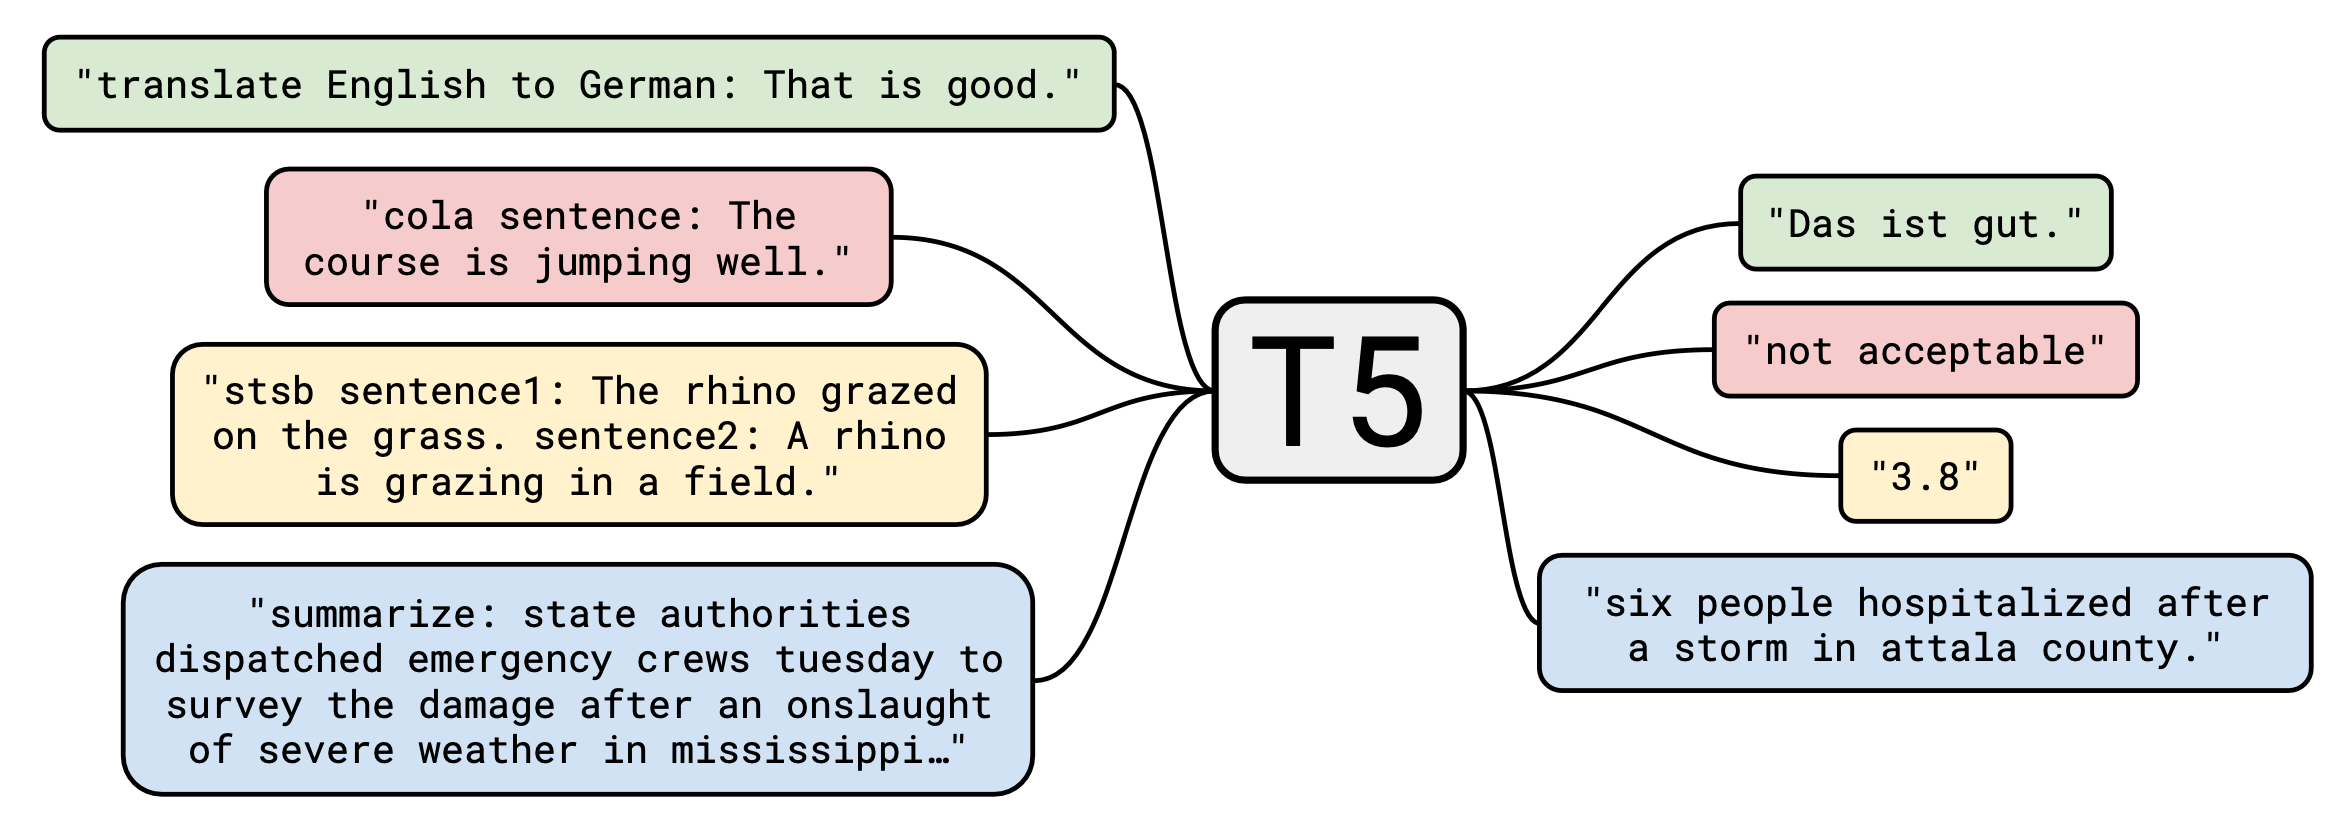
\includegraphics[width=\textwidth]{t5}
	\caption{A diagram of the T5 text-to-text framework. Every task -- including translation, question answering, and classification -- is cast as feeding the model text as input and training it to generate some target text. This approach allows the same model, loss function, hyperparameters, etc., to be used across diverse tasks. Source: \textcite{raffel2023exploring}.}
	\label{fig:t5-t2t}
\end{figure}

T5 demonstrated its prowess across a range of benchmarks, setting new standards in the field of NLP~\cite{raffel2023exploring}.
It's built on the transformer model, similar to its predecessors, BERT and GPT. It leverages the effective self-attention mechanism for processing data sequences.
The model is designed to handle various tasks without needing task-specific architectural modifications.
It uses a unified text-to-text framework, where tasks are converted into a format where the input and output are always text strings.
T5 is pre-trained on a multitask mixture of unsupervised and supervised tasks, utilising a large-scale dataset known as "C4"~\footnote{Colossal Clean Crawled Corpus}.

T5's approach simplifies integrating new tasks into the model's training regime, as they only need to be reformulated into the text-to-text format.
While T5's unified approach offers considerable advantages, it might not be optimal for all types of tasks.
Some tasks could potentially benefit from more specialised model architectures or formats.
The training process for T5 is resource-intensive, requiring substantial computational power, which could be a limiting factor for smaller organisations or independent researchers.
As with other large language models, T5's outputs can sometimes include biases in the training data, necessitating careful monitoring and potential post-hoc adjustments.

\subsection{GPT Series}
\label{subsec:gpt-series}

Developed by OpenAI, the GPT series has been at the forefront of LLM research.
The original GPT model, introduced in 2018, laid the groundwork with its transformer-based architecture, significantly improving previous models' understanding of context and generating text.
It was developed based on a generative, decoder-only Transformer architecture, and it adopted a hybrid approach of unsupervised pre-training and supervised fine-tuning.

GPT-2~\cite{radford2019language}, released in 2019, expanded on this with 1.5 billion parameters and was trained with a large webpage dataset, WebText, demonstrating unprecedented text generation capabilities.

The subsequent GPT-3 model, unveiled in 2020, further pushed the boundaries with 175 billion parameters, showcasing remarkable abilities in generating human-like text, performing language translation, question-answering, and more without task-specific training.
In the research paper on GPT-3~\cite{brown2020language}, the authors explained the concept known as in-context learning (ICL). This approach enables Large Language Models (LLMs) to function in few-shot or zero-shot scenarios.
ICL empowers LLMs to comprehend tasks when they are described using natural language.
This method aligns LLMs' pre-training and application phases under a unified framework. During pre-training, the model predicts subsequent text sequences based on the prior context.
In contrast, during in-context learning, the model generates the appropriate solution to a task in the form of a text sequence using the provided task instructions and examples.

The GPT series is based on the transformer architecture by \textcite{vaswani2023attention}.
This architecture leverages self-attention mechanisms to process input data, which allows the model to weigh the importance of different words within the input context, enhancing its ability to understand and generate language.
GPT models are characterized by their stacked transformer blocks, which consist of multi-headed self-attention layers followed by fully connected feed-forward neural networks.
The series has seen an exponential increase in the number of parameters: GPT with 110 million, GPT-2 with 1.5 billion, and GPT-3 with 175 billion parameters.

GPT models exhibit a remarkable ability to generate coherent and contextually relevant text, simulating human-like writing styles.
They demonstrate strong performance in a wide array of NLP tasks without task-specific data training, showcasing their versatility in few-shot, one-shot, or zero-shot learning scenarios.
The architecture's scalability has shown that larger models tend to exhibit better performance and capture subtler patterns in data.

One significant criticism is their data-hungry nature, requiring vast amounts of text data for training, which raises concerns about environmental impact and computational costs.
The models can sometimes generate plausible but factually incorrect or nonsensical information, a phenomenon often referred to as \enquote{hallucination}.
The black-box nature of these models poses challenges in interpretability and transparency, making it difficult to understand how decisions are made or how to correct biases.

GPT-3 demonstrated surprising emergent behaviours, such as improved reasoning, problem-solving, and creative writing, which were not explicitly programmed or observed in their predecessors.
These abilities suggest that scaling up model size can lead to qualitative changes in how models understand and interact with language, although the relationship is not yet fully understood.
OpenAI has explored two major approaches to further improving the GPT-3 model, i.e., training on code data and alignment with human preference, which are detailed as follows:
\begin{enumerate}
	\item \textbf{Training on code data:} {
		      This approach involves fine-tuning the model on a diverse set of programming tasks, such as code completion, code generation, and code summarization.
		      The model is trained on a large corpus of code data, which includes code snippets, programming languages, and software development documentation.
		      The goal is to improve the model's understanding of programming languages and its ability to generate code, thereby enhancing its performance on programming-related tasks.
	      }
	\item \textbf{Alignment with human preference:} {
	      This approach involves training the model to generate outputs that align with human preferences and values and can be dated back to a work that applied reinforcement learning (RL) \textcite{christiano2017deep} (similar to the reward training step in the aligning algorithm of InstructGPT.
	      }
\end{enumerate}

\subsubsection{GTP-4}
\label{subsubsec:gpt-4}

GPT-4~\cite{openai2024gpt4}, the successor to GPT-3, marks a further advancement in the GPT series developed by OpenAI. While specific details about GPT-4's architecture and capabilities are proprietary, it is known to build upon the foundational concepts of its predecessors, emphasizing scale, capability, and efficiency.
GPT-4 is a multimodal model which can accept image and text inputs and produce text outputs.
Such models are an important area of study as they have the potential to be used in a wide range of applications, such as dialogue systems, text summarization, and machine translation.

\begin{table}[h!]
	\centering
	\label{tab:gpt4_example}
	\begin{tabular}{@{}m{2cm}@{}m{10cm}@{}}
		User  & What is funny about this image? Describe it panel by panel.                                                                                                                                                                                                                                                                                                                                         \\
		      & 
\includegraphics[width=10cm]{gpt4}                                                                                                                                                                                                                                                                                                                                                                  \\
		      &                                                                                                                                                                                                                                                                                                                                                                                                     \\
		GPT-4 &
		\begin{tabular}[t]{@{}m{10cm}@{}}
			The image shows a "Lightning Cable" adapter package with three panels.                                                                                                                                                                                                                                                                                                                                      \\
			Panel 1: A smartphone with a VGA connector (a large, blue, 15-pin connector typically used for computer monitors) plugged into its charging port.                                                                                                                                                                                                                                                           \\
			Panel 2: The package for the "Lightning Cable" adapter with a picture of a VGA connector on it.                                                                                                                                                                                                                                                                                                             \\
			Panel 3: A close-up of the VGA connector with a small Lightning connector (used for charging iPhones and other Apple devices) at the end.                                                                                                                                                                                                                                                                   \\
			The humour in this image comes from the absurdity of plugging a large, outdated VGA connector into a small, modern smartphone charging port.                                                                                                                                                                                                                                                                \\
			The model can grasp the context of the image and provide a detailed description of each panel, highlighting the humour in the visual juxtaposition of old and new technology\footnote{There are literal websites that explain jokes, and why something is funny. So, we truly don’t know whether LLM's explanation of the joke is coming from the trueunderstanding of language or from those retrievals.}. \\
		\end{tabular} \\
	\end{tabular}
	\caption{Example prompt demonstrating GPT-4's visual input capability. The prompt consists of a question about an image with multiple panels.}
\end{table}

On the MMLU benchmark~\cite{hendrycks2021measuring}, an English-language suite of multiple-choice questions covering 57 subjects, GPT-4 outperforms existing models by a considerable margin in English and demonstrates strong performance in other languages.
GPT-4 development was enabled by deep learning infrastructure and optimization methods that behave predictably across various scales.
The approach allowed the authors to predict the expected performance of GPT-4 (based on small runs trained similarly), which was tested against the final run, to increase confidence in the training.
The primary reason is that extensive model-specific tuning is not feasible for very large training runs.

The prediction GPT-4's final loss was predicted by fitting a scaling law with an irreducible loss term (as in~\textcite{henighan2020scaling}):

\begin{equation}
	L(C) = aC^b + c
	\label{eq:gpt4-scaling-law}
\end{equation}

\noindent from models trained using the same methodology but using at most 10,000\texttimes less compute than GPT-4.
The fitted scaling law predicted GPT-4's final loss with high accuracy.
In addition to predicting the final loss, a metric of capability was also predicted.
One such metric is the pass rate on HumanEval dataset~\cite{chen2021evaluating}, which measures the ability to write Python functions of various complexity.
The approximate power law relationship is

\begin{equation}
	E_P [\log{pass\_rate(C)}] = \alpha \times C^{-k}
	\label{eq:gpt4-pass-rate}
\end{equation}

\noindent where k and \(\alpha\) are positive constants, and P is a subset of problems in the dataset.

GPT-4 accepts prompts consisting of images and text, which lets the user specify any vision or language task in parallel to the text-only setting.
Specifically, the model generates text outputs, given inputs consisting of arbitrarily interlaced text and images.
Despite its capabilities, GPT-4 has similar limitations to earlier GPT models: it is not fully reliable (e.g.\ can suffer from \enquote{hallucinations}), has a limited context window, and does not learn from experience.
Care should be taken when using the outputs of GPT-4, particularly in contexts where reliability is important.

\subsection{Llama}
\label{subsec:llama}

Llama~\footnote{Large Language Model Meta AI} is a language model developed by Meta AI, designed to be a versatile and efficient foundation for a wide range of natural language processing (NLP) tasks.
Llama is built on a transformer architecture~\cite{vaswani2023attention}, similar to other large language models, with a range from 7B to 65B parameters.
Main differences between Llama and original Transformer architecture~\cite{vaswani2023attention} are the following:
\begin{enumerate}
	\item \textbf{Pre-normalization\footnote{Inspired by GTP-3 model}} {Llama uses pre-normalization\footnote{See Section \ref{subsubsec:normalization}}, which means that the normalization layer is placed before the self-attention and feed-forward layers.
		      Pre-normalization has improved training stability and convergence in large language models, making it a popular choice for many state-of-the-art models.
	      }
	\item \textbf{SwiGLU activation function\footnote{Inspired by PaLM model}} {Llama uses the SwiGLU\footnote{See Section \ref{subsubsec:activation-functions}} activation function by \textcite{shazeer2020glu}, which is a variant of the Gated Linear Unit (GLU) activation function.
		      SwiGLU has been shown to improve the performance of large language models by enhancing the flow of information through the network.
	      }
	\item \textbf{Rotary Embeddings\footnote{Inspired by GPTNeo model}} {Llama uses rotary embeddings by \textcite{su2021roformer}, which are a type of positional encoding that helps the model capture long-range dependencies in the input data.
	      }
\end{enumerate}

\begin{table}[ht]
	\centering
	\begin{tabular}{@{}ccccccc@{}}
		\toprule
		params & dimension & n heads & n layers & learning rate          & batch size & n tokens \\
		\midrule
		6.7B   & 4096      & 32      & 32       & \(3.0 \times 10^{-4}\) & 4M         & 1.0T     \\
		13.0B  & 5120      & 40      & 40       & \(3.0 \times 10^{-4}\) & 4M         & 1.0T     \\
		32.5B  & 6656      & 52      & 60       & \(1.5 \times 10^{-4}\) & 4M         & 1.4T     \\
		65.2B  & 8192      & 64      & 80       & \(1.5 \times 10^{-4}\) & 4M         & 1.4T     \\
		\bottomrule
	\end{tabular}
	\caption{Llama model sizes, architectures, and optimization hyper-parameters. Source: \textcite{touvron2023llama}.}
	\label{tab:llama-model-params}
\end{table}

Based on the Llama paper by \textcite{touvron2023llama}, even though Llama \textsubscript{13B} is smaller than many competitors, it outperforms GPT-3 on most benchmarks, and the 65B model is competitive with the best large language models available, such as Chinchilla and PaLM-540B, despite being x10 smaller (as shown in Table~\ref{tab:llama-zero-shot-performance}).

\begin{table}[htbp]
	\centering
	\scriptsize
	\begin{tabularx}{\textwidth}{@{}lXXXXXXXXX@{}}
		\toprule
		Model      & Params & BoolQ & PIQA & SIQA & HellaSwag & WinoGrande & ARC-e & ARC-c & OBQA \\
		\midrule
		GPT-3      & 175B   & 60.5  & 81.0 & -    & 78.9      & 70.2       & 68.8  & 51.4  & 57.6 \\
		Gopher     & 280B   & 79.3  & 81.8 & 50.6 & 79.2      & 70.1       & -     & -     & -    \\
		Chinchilla & 70B    & 83.7  & 81.8 & 51.3 & 80.8      & 74.9       & -     & -     & -    \\
		PaLM       & 62B    & 84.8  & 80.5 & -    & 79.7      & 77.0       & 75.2  & 52.5  & 50.4 \\
		PaLM-cont  & 62B    & 83.9  & 81.4 & -    & 80.6      & 77.0       & -     & -     & -    \\
		PaLM       & 540B   & 88.0  & 82.3 & -    & 83.4      & 81.1       & 76.6  & 53.0  & 53.4 \\
		\addlinespace
		Llama      & 7B     & 76.5  & 79.8 & 48.9 & 76.1      & 70.1       & 72.8  & 47.6  & 57.2 \\
		Llama      & 13B    & 78.1  & 80.1 & 50.4 & 79.2      & 73.0       & 74.8  & 52.7  & 56.4 \\
		Llama      & 33B    & 83.1  & 82.3 & 50.4 & 82.8      & 76.0       & 80.0  & 57.8  & 58.6 \\
		Llama      & 65B    & 85.3  & 82.8 & 52.3 & 84.2      & 77.0       & 78.9  & 56.0  & 60.2 \\
		\bottomrule
	\end{tabularx}
	\caption{Zero-shot performance on Common Sense Reasoning tasks. Source: \textcite{touvron2023llama}.}
	\label{tab:llama-zero-shot-performance}
\end{table}

The Llama models were trained exclusively on publicly available data, setting them apart from other models that rely on proprietary datasets~\footnote{Such as "Books --- 2TB" or "Social media conversations"}.
The dataset is a mixture of several sources (webpages, books, scientific data and code) as reported in Table~\ref{tab:llama-pretraining-data}.

\begin{table}[h!]
	\centering
	\begin{tabularx}{\textwidth}{Xlccc}
		\hline
		\textbf{Dataset} & \textbf{Classification} & \textbf{Sampling prop.} & \textbf{Epochs} & \textbf{Disk size} \\
		\hline
		CommonCrawl      & Webpages                & 67.0\%                  & 1.10            & 3.3 TB             \\
		C4               & Web                     & 15.0\%                  & 1.06            & 783 GB             \\
		Github           & Code                    & 4.5\%                   & 0.64            & 328 GB             \\
		Wikipedia        & Webpages                & 4.5\%                   & 2.45            & 83 GB              \\
		Books            & Books                   & 4.5\%                   & 2.23            & 85 GB              \\
		ArXiv            & Scientific Data         & 2.5\%                   & 1.06            & 92 GB              \\
		StackExchange    & Conversation Data       & 2.0\%                   & 1.03            & 78 GB              \\
		\hline
	\end{tabularx}
	\caption{Pre-training data. Data mixtures used for pre-training for each subset, the table reports the sampling proportion, number of epochs performed on the subset when training on 1.4T tokens, and disk size. The pre-training runs on 1T tokens have the same sampling proportion. Source: \textcite{touvron2023llama}.}
	\label{tab:llama-pretraining-data}
\end{table}

Llama models were designed with efficiency in mind, both in training and inference, allowing even the 13B parameter model to run on a single GPU\@.
A synthetic view of the Llama model family parameters is reported in Table~\ref{tab:llama-model-params}.
The optimizer used during the training is the same AdamW with the following hyper-parameters: $\beta_1=0.9, \beta_2=0.95, eps=10^{-5}$, a weight decay of 0.1, gradient clipping of 1.0, a cosine learning rate schedule and a warmup of 2000 steps.

\textcite{touvron2023llama} acknowledges the presence of biases and toxicity in the models due to the nature of web data and evaluates these aspects using benchmarks from the responsible AI community.

\subsubsection{Llama 2}
\label{subsubsec:llama-2}

Llama 2~\cite{touvron2023llama2} is a continuation of the Llama series, developed by Meta AI, released in scale from 7B to 70B parameters.
The pre-training data of the Llama2 model is a new mix of data from publicly available sources.
The training corpus is 40\% larger than the one used for Llama 1, and it is composed of a mix of text and a percentage of code data that is roughly 8\% of the total.
The exact composition of the data mix is not disclosed, but the code percentage is reported in the caption of the Table~\ref{tab:llama2-pretraining-data} extracted from the original paper~\cite{touvron2023llama2}.
The pre-training selection focuses on addressing biases and toxicity recognised in the previous version of the model.

\begin{table}[h!]
	\centering
	\begin{tabularx}{\textwidth}{XclcX}
		\hline
		\textbf{Language} & \textbf{Percent} & \textbf{Language} & \textbf{Percent} \\
		\hline
		en                & 89.70\%          & uk                & 0.07\%           \\
		unknown           & 8.38\%           & ko                & 0.06\%           \\
		de                & 0.17\%           & ca                & 0.04\%           \\
		fr                & 0.16\%           & sr                & 0.04\%           \\
		sv                & 0.15\%           & id                & 0.03\%           \\
		zh                & 0.13\%           & cs                & 0.03\%           \\
		es                & 0.13\%           & fi                & 0.03\%           \\
		ru                & 0.13\%           & hu                & 0.03\%           \\
		nl                & 0.12\%           & no                & 0.03\%           \\
		it                & 0.11\%           & ro                & 0.03\%           \\
		ja                & 0.10\%           & bg                & 0.02\%           \\
		pl                & 0.09\%           & da                & 0.02\%           \\
		pt                & 0.09\%           & sl                & 0.01\%           \\
		vi                & 0.08\%           & hr                & 0.01\%           \\
		\hline
	\end{tabularx}
	\caption{Language distribution in pretraining data with percentage $\geq$ 0.005\%. Most data is in English, meaning that LLaMA 2 will perform best for English-language use cases. The large unknown category is partially made up of programming code data.}
	\label{tab:llama2-pretraining-data}
\end{table}

Llama 2 adopts most of the pretraining settings and model architecture from Llama 1, including the standard transformer architecture, pre-normalization using RMSNorm, the SwiGLU activation function, and rotary positional embeddings.
The optimizer used during the training is the same AdamW with the following hyper-parameters: $\beta_1=0.9, \beta_2=0.95, eps=10^{-5}$, a weight decay of 0.1, gradient clipping of 1.0, a cosine learning rate schedule and a warmup of 2000 steps.
The primary architectural differences from Llama 1 include increased context length and grouped-query attention (GQA).

\subsubsection{Code Llama}
\label{subsubsec:code-llama}

Code Llama~\cite{roziere2024codellamaopenfoundation} is a family of large language models for code generation based on Llama 2 providing infilling\footnote{With the terms infilling or code completion, we refer to the process of generating code snippets that complete a given code fragment.} capabilities, support
for large input contexts and zero-shot instruction following ability for programming tasks.
It comes in three flavours: the vanilla model, the Python specialized model, and the instruction-following model with 7B, 13B, 34B, and 70B parameters each (see Figure~\ref{fig:code-llama}).

\begin{figure}[h!]
	\centering
	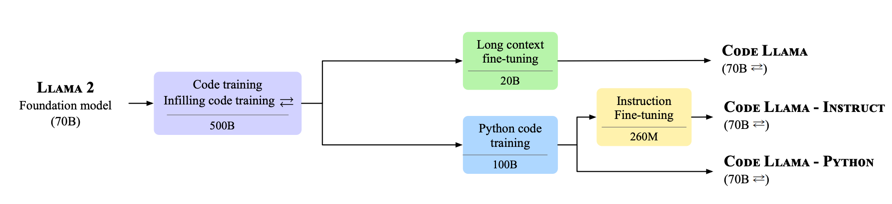
\includegraphics[width=0.9\textwidth]{codellama-pipeline}
	\caption{The Code Llama 70B specialization pipeline. The different fine-tuning stages are annotated with the number of tokens seen during training. Infilling-capable models are marked with the $\rightleftarrows$ symbol. Source: \textcite{roziere2024codellamaopenfoundation}.}
	\label{fig:code-llama}
\end{figure}

While most of the code generation models are trained on code only, Code Llama was fine-tuned starting from Llama 2, which was trained on general-purpose text and code data.
The comparison in \textcite{roziere2024codellamaopenfoundation} shows that initializing from Llama 2 leads to better performance on code generation tasks than initializing from a code-only model for a given budget as shown in Figure~\ref{fig:code-llama-comparison}.
Code Llama was fine-tuned on 500B extra tokens consisting mostly of code data (85\%).

\begin{figure}[ht!]
	\centering
	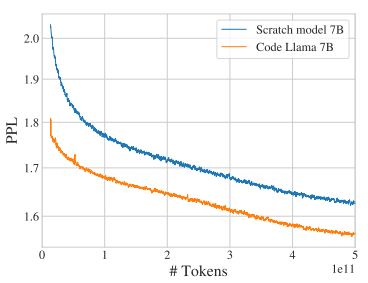
\includegraphics[width=0.7\textwidth]{codellama-loss}
	\caption{Comparison of Code Llama models versus an identical model trained from scratch. Source: \textcite{roziere2024codellamaopenfoundation}.}
	\label{fig:code-llama-comparison}
\end{figure}

\subsubsection{Llama 3}
\label{subsubsec:llama-3}

Llama 3~\cite{llama3} is a continuation of the Llama series, developed by Meta AI, with different model sizes: 8B, 70B, and 405B parameters.

Llama 3 uses a standard, dense Transformer architecture.
It does not deviate significantly from Llama and Llama 2 in terms of model architecture; therefore performance gains are primarily driven by improvements in data quality and diversity as well as by increased training scale.
Compared to Llama 2, Llama 3 has a few small changes in the model architecture:
\begin{enumerate}
	\item grouped query attention (GQA) with 8 key-value heads to improve inference speed and to reduce the size of key-value caches during decoding
	\item an attention mask that prevents self-attention between different documents within the same sequence.
	      This change has limited impact during standard pre-training, but it's important in continued pre-training on very long sequences.
	\item a vocabulary with 128K tokens.
	      Compared to the Llama 2 tokenizer, the new tokenizer improves compression rates on a sample of English data from 3.17 to 3.94 characters per token.
	\item the RoPE base frequency hyper-parameter increased to 500,000 to support longer contexts.
\end{enumerate}
A summary of the key hyper-parameters of Llama 3 is shown in Table~\ref{tab:llama3-hyperparameters}.

\begin{table}[h!]
	\centering
	\caption{Overview of the key hyperparameters of Llama 3. We display settings for 8B, 70B, and 405B language models.}
	\begin{tabularx}{\textwidth}{Xccc}
		\textbf{}                      & \textbf{8B}               & \textbf{70B}              & \textbf{405B}             \\
		\textbf{Layers}                & 32                        & 80                        & 126                       \\
		\textbf{Model Dimension}       & 4096                      & 8192                      & 16384                     \\
		\textbf{FFN Dimension}         & 14336                     & 28672                     & 53248                     \\
		\textbf{Attention Heads}       & 32                        & 64                        & 128                       \\
		\textbf{Key/Value Heads}       & 8                         & 8                         & 8                         \\
		\textbf{Peak Learning Rate}    & $3 \times 10^{-4}$        & $1.5 \times 10^{-4}$      & $8 \times 10^{-5}$        \\
		\textbf{Activation Function}   & SwiGLU                    & SwiGLU                    & SwiGLU                    \\
		\textbf{Vocabulary Size}       & 128,000                   & 128,000                   & 128,000                   \\
		\textbf{Positional Embeddings} & RoPE ($\theta = 500,000$) & RoPE ($\theta = 500,000$) & RoPE ($\theta = 500,000$) \\
		\hline
	\end{tabularx}
	\caption{Overview of the key hyperparameters of Llama 3}
	\label{tab:llama3-hyperparameters}
\end{table}

The authors improved the quantity and quality of the data we used for pre-training and post-training compared to prior versions of Llama.
These improvements include developing more careful pre-processing and curation pipelines for pre-training data and more rigorous quality assurance and filtering approaches for post-training data.
The pre-training corpus consists of about 15T tokens, which is about 50% larger than the one used for Llama 2.
It contains roughly 50\% of tokens corresponding to general knowledge, 25\% of mathematical and reasoning tokens, 17\% code tokens, and 8\% multilingual tokens~\cite{llama3}.
The resulting models have a rich set of capabilities.
They can answer questions in at least eight languages, write high-quality code, solve complex reasoning problems, and use tools out-of-the-box or in a zero-shot way


\subsection{Gemma}
\label{subsec:gemma}

The recent development in the domain of Natural Language Processing has seen Google's introduction of a new family of models named Gemma~\cite{gemma_google_ai, gemmateam2024gemma}.
Derived from the same research lineage as the renowned Gemini models, Gemma is a testament to the rapid advancements in lightweight, high-performance language models designed for a broad spectrum of computational environments.

Gemma is built upon a transformer-based architecture by \textcite{vaswani2023attention}, optimized to deliver state-of-the-art performance with a fraction of the parameter count typically seen in large language models (LLMs).
Notable enhancements include the adoption of Multi-Query Attention, RoPE embeddings, GeGLU activations, and RMSNorm, indicating an evolution of the original transformer architecture.
The family comprises two main configurations: Gemma 2B and Gemma 7B, available in pre-trained and instruction-tuned variants.
The design philosophy targets efficient deployment across diverse hardware platforms, including but not limited to mobile devices, laptops, desktop computers, and servers.

\begin{figure}[ht!]
	\centering
	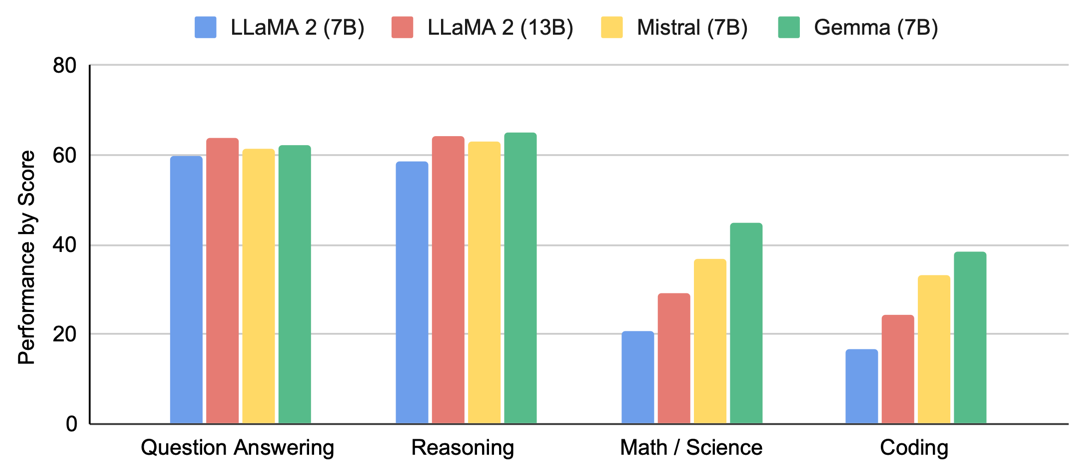
\includegraphics[width=0.9\textwidth]{gemma_comparison2}
	\caption{Gemma models exhibit superior performance in language understanding and reasoning tasks compared to larger models. Source: \textcite{gemmateam2024gemma}.}
	\label{fig:gemma-comparison2}
\end{figure}

In comparative benchmarks, Gemma models have demonstrated capabilities that exceed those of larger parameter models, such as Llama 2 (13B), indicating a significant efficiency in parameter utilization.
Improvements are particularly evident in language understanding and reasoning tasks where Gemma models have been pitted against their contemporaries.

One prominent strength of Gemma models is their deployment efficiency, which democratizes access to state-of-the-art NLP tools.
The models are designed to be run on common developer hardware, eschewing the need for specialized AI accelerators.

\begin{figure}[ht!]
	\centering
	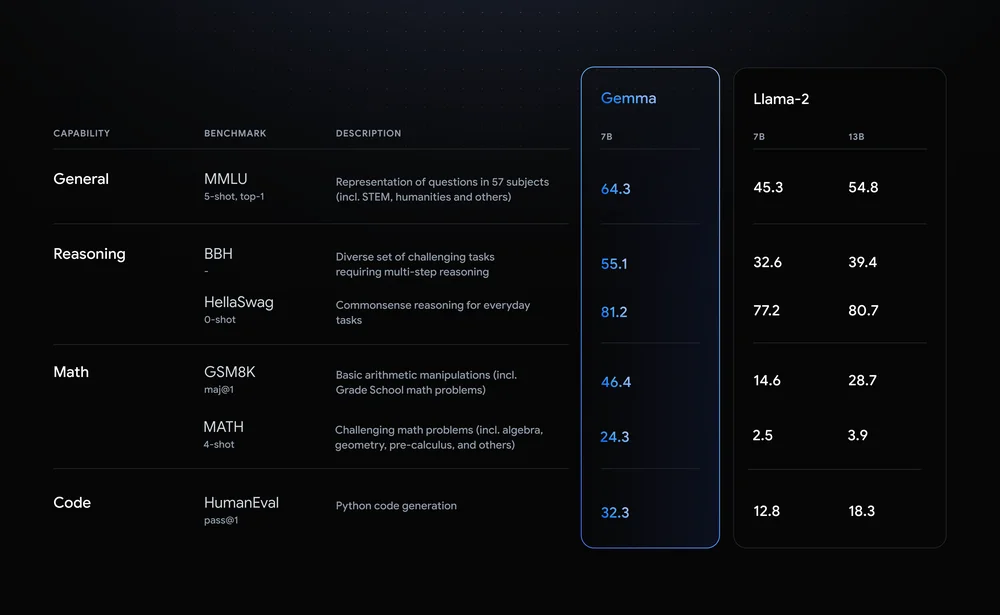
\includegraphics[width=\textwidth]{gemma_comparison}
	\caption{Gemma models are designed to be lightweight and efficient, making them accessible to a wide range of developers and applications. Source: \textcite{gemma_google_ai}.}
	\label{fig:gemma-comparison}
\end{figure}

Despite their efficiencies, the Gemma models are not without limitations.
While the reduced parameter count is advantageous for accessibility and computational efficiency, it may impact performance in complex NLP tasks that can benefit from larger models.
Additionally, ethical considerations, such as bias in language models, remain an area of concern and active development.

Google has emphasized the responsible development of AI, which is evident in Gemma's design.
Techniques to mitigate sensitive data inclusion and reinforcement learning from human feedback are incorporated to ensure the models' outputs adhere to safety standards.
Moreover, Google's release includes a Responsible Generative AI Toolkit to aid developers in prioritizing the creation of ethical AI applications.


\section{Specialized Large Language Models}
\label{sec:applications-of-large-language-models}

Specialized Large Language Models (LLMs) are model checkpoints refined for particular fields or tasks, such as healthcare and finance.
The existing domain-specific models are developed by pre-training on specialized datasets~\cite{luo2022biogpt,bolton2023biomedlm, taylor2022galactica}), by adapting a very large general-purpose model to domain-specific tasks~\cite{singhal2022large, liang2022holistic}, or mixing both approaches~\cite{wu2023bloomberggpt}.
These models serve as domain-specific problem solvers and are evaluated based on general competencies, such as fundamental complex reasoning, and more nuanced capabilities, like alignment with human intent, as well as their performance in areas specific to their application.
To accurately measure their efficacy, specialized benchmarks are developed that cater to these distinct sectors.
These tailored benchmarks are then employed in conjunction with broader assessments to provide a holistic and focused evaluation of the models' capabilities.
The following sections highlight some of LLMs' key applications and their impact on different sectors, from healthcare to finance and education to research.

\subsection{LLMs in Healthcare}
\label{subsec:llms-in-healthcare}
The intersection of artificial intelligence (AI) and healthcare has precipitated unparalleled advances in the provision of medical services, diagnosis, treatment, and patient care.
Central to these advancements are Large Language Models (LLMs), which have been instrumental in catalyzing transformative changes across the healthcare sector:

\begin{enumerate}
	\item \textbf{Medical image analysis:}{
		      Large Language Models (LLMs) have been integrated with medical imaging technologies to enhance diagnostic accuracy and efficiency.
		      By analyzing radiological images and clinical reports, LLMs can assist radiologists in interpreting images, identifying abnormalities, and providing diagnostic insights.
		      These models leverage their natural language processing capabilities to extract information from textual reports and correlate it with visual data, thereby augmenting the diagnostic process~\cite{li2021survey, zhang2021medical}.
	      }

	\item \textbf{Clinical Decision Support:}{
		      LLMs have been pivotal in augmenting clinical decision support systems (CDSS). By analyzing patient data and medical literature, LLMs assist clinicians in diagnosing conditions, suggesting treatment options, and predicting patient outcomes. For instance, models like BERT and its derivatives have been fine-tuned on medical corpora, yielding tools that can parse clinical notes, interpret lab results, and provide evidence-based recommendations~\cite{alsentzer2019publicly}.
	      }

	\item \textbf{Medical Documentation and Coding:}{
		      The onus of medical documentation and billing has traditionally been a significant administrative burden for healthcare providers. LLMs have demonstrated the ability to streamline these processes by automating the translation of clinical dialogue and notes into structured electronic health records (EHRs) and accurately coding medical procedures, thus mitigating errors and saving time~\cite{shickel2018deep}.
	      }

	\item \textbf{Drug Discovery and Development:}{
		      In the domain of pharmaceuticals, LLMs have expedited the drug discovery and development pipelines. By mining through vast chemical libraries and medical databases, these models facilitate the identification of potential drug candidates and the repurposing of existing drugs for new therapeutic uses~\cite{zhavoronkov2019deep}.
	      }

	\item \textbf{Personalized Medicine:}{
		      Personalized medicine, which tailors treatment to individual patient characteristics, has benefited from LLMs by generating patient-specific models that predict disease susceptibility and drug response. This personalization extends to creating tailored health interventions based on patient history and genetic information~\cite{hamburg2010path}.
	      }

	\item \textbf{Patient Engagement and Self-Management:}{
		      LLMs are also revolutionizing patient engagement by powering intelligent virtual health assistants capable of providing information, reminders, and motivational support for chronic disease self-management. These AI assistants interact with patients in natural language, thus fostering an environment conducive to patient education and adherence to treatment regimens~\cite{kocaballi2019personalization}.
	      }
\end{enumerate}

Despite these strengths, LLMs face significant challenges within healthcare applications.
Concerns regarding patient privacy, data security, and the need for explainability in AI-driven decisions are paramount~\cite{beam2018big}.
Additionally, biases inherent in training data can perpetuate disparities in patient care, necessitating rigorous validation and fairness assessments before clinical deployment~\cite{chen2019single}.

Large Language Models represent a transformative force in healthcare, enhancing efficiency, accuracy, and personalization in various medical domains.
Their integration into clinical practice must be pursued with diligent oversight to navigate ethical considerations and ensure equitable and safe applications.

\subsubsection{Med-PaLM}
\label{subsubsec:med-palm}

One of the most advanced LLMs for healthcare is Med-PaLM, a derivative of the PaLM (540B) model developed by Google and its instruction-tuned variant, Flan-PaLM. Using a combination of few-shot~\cite{brown2020language}), chain-of-thought (CoT) (\textcite{wei2022chain}), and self-consistency (\textcite{wang2022self} prompting strategies, Flan-PaLM achieved state-of-the-art accuracy on every MultiMedQA \footnote{Stands for a multi-domain medical question answering benchmark. It has been designed to evaluate the performance of LLMs in the healthcare sector.
	This benchmark likely encompasses a wide range of medical questions, covering various disciplines, conditions, and scenarios that medical professionals encounter.} multiple-choice dataset (MedQA, MedMCQA, PubMedQA, MMLU clinical topics and a newly introduced dataset, HealthSearchQA, which consists of commonly searched health questions).

\begin{table}[!h]
	\centering
	\begin{tabular}{@{}lc@{}}
		\toprule
		Model (number of parameters) & MedQA (USMLE) Accuracy \% \\
		\midrule
		Flan-PaLM (540 B)            & 67.6                      \\
		PubMedGPT (2.7 B)            & 50.3                      \\
		DRAGON (360 M)               & 47.5                      \\
		BioLinkBERT (340 M)          & 45.1                      \\
		Galactica (120 B)            & 44.4                      \\
		PubMedBERT (100 M)           & 38.1                      \\
		GPT-Neo (2.7 B)              & 33.3                      \\
		\bottomrule
	\end{tabular}
	\caption{Performance comparison of different models on the MedQA (USMLE) benchmark. Source: \textcite{singhal2022large}.}
	\label{tab:medqa_performance}
\end{table}

Despite these remarkable results, human evaluation reveals key gaps in Flan-PaLM responses and remains inferior to clinicians~\cite{singhal2022large}.
To resolve this issue, researchers introduced "instruction tuning"\footnote{See Section \ref{subsec:instruction-tuning}} to align the Flan-PaLM model to the medical domain.
Thus, Instruction tuning can be seen as a lightweight way (data-efficient, parameter-efficient, compute-efficient during training and inference) of training a model to follow instructions in one or more domains.
Instruction tuning adapted LLMs to follow better the specific type of instructions used in the family of medical datasets.
The result was Med-PaLM, a model that significantly reduces the gap (or even compares favourably) to clinicians on several evaluation axes, according to clinicians and lay users.

\begin{figure}[h!]
	\centering
	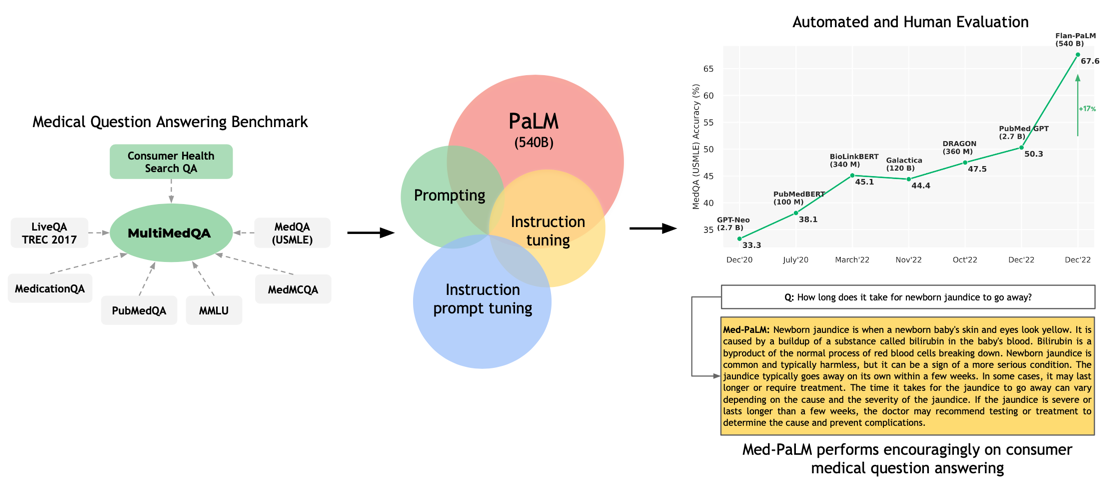
\includegraphics[width=\textwidth]{flan-palm}
	\caption{Large Language Models (LLMs) have revolutionized healthcare by enhancing diagnostic accuracy, clinical decision support, and patient engagement. Source: \textcite{singhal2022large}.}
	\label{fig:llm-healthcare}
\end{figure}

\subsection{LLMs in Finance}
\label{subsec:llms-in-finance}

There has been growing interest in applying NLP to various financial tasks, including sentiment analysis, question answering, and stock market prediction.
Despite the extensive research into general-domain LLMs and their immense potential in finance, Financial LLM (Fin-LLM) research remains limited, and the field of financial LLMs is at an early stage~\cite{lee2024survey}.
An overview of the evolution of selected PLM/LLM releases from the general domain to the financial domain is shown in Figure~\ref{fig:llm-finance}.

\begin{figure}[h]
	\centering
	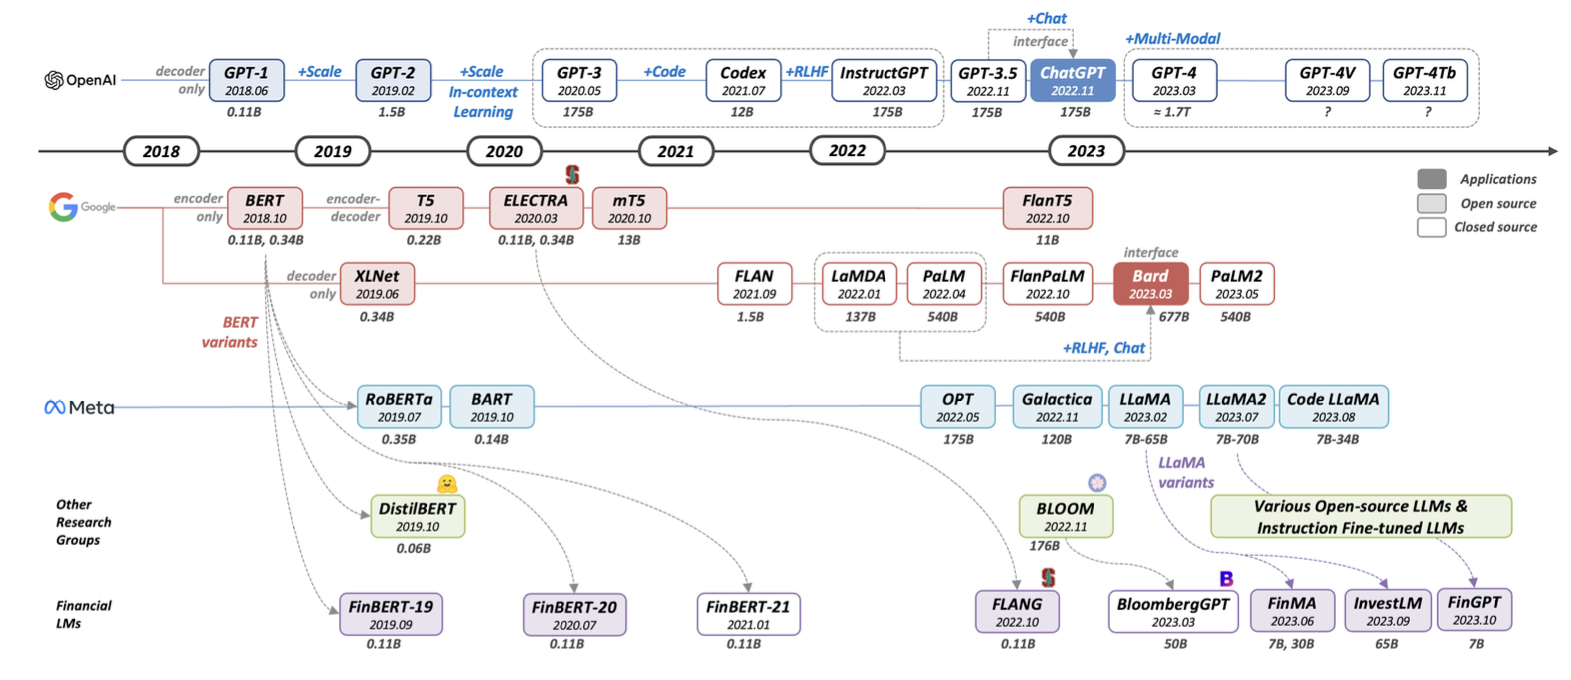
\includegraphics[width=\textwidth]{FinLLMs}
	\caption{Timeline showing the evolution of selected PLM/LLM releases from the general domain to the financial domain. Source: \textcite{lee2024survey}.}
	\label{fig:llm-finance}
\end{figure}

Some of these models have demonstrated the potential of LLMs to understand complex financial jargon, generate insights, predict market trends, and enhance customer interaction with unprecedented precision and relevance.

Here are some key applications of LLMs in the financial sector:

\begin{enumerate}
	\item \textbf{Algorithmic Trading:}
	      {LLMs analyze vast amounts of unstructured data, including news articles, financial reports, and social media, to gauge market sentiment and predict stock price movements.
		      Their predictive insights enable more informed algorithmic trading strategies~\cite{buehler2018deep}.}

	\item \textbf{Risk Management:}
	      {In risk management, LLMs contribute by parsing and interpreting complex regulatory documents, identifying potential compliance risks, and offering actionable insights to mitigate financial and reputational risks~\cite{li2020natural}.}

	\item \textbf{Customer Service Automation:}
	      {Financial institutions leverage LLMs to power chatbots and virtual assistants, providing real-time, personalized customer service. These AI-driven systems can handle inquiries, execute transactions, and offer financial advice, enhancing customer experience and operational efficiency~\cite{pal2021enhancing}.}

	\item \textbf{Fraud Detection:}
	      {LLMs enhance fraud detection systems by analyzing transactional data and customer communication to identify patterns indicative of fraudulent activities, thereby bolstering the security of financial transactions~\cite{smith2019improving}.}
\end{enumerate}

Some of the models in Figure~\ref{fig:llm-finance} have augmented the accuracy and efficiency of financial analyses and expedited the decision-making processes, enabling more timely and informed decisions.
Additionally, their role in risk management is noteworthy, where their data processing and analytical prowess help identify potential risks and adherence issues more effectively than traditional methodologies~\cite{buehler2018deep}.

Despite their potential, LLMs in finance face challenges, including data privacy concerns, the need for interpretability in model decisions, and the risk of perpetuating biases from training data.
Ensuring these models adhere to ethical standards and regulatory compliance is paramount~\cite{jones2020ethical, buehler2018deep}.

Let's delve deeper into the techniques used to adapt LLMs for the financial sector to enhance their performance on finance-specific tasks~\cite{lee2024survey}.
These techniques enhance the models' understanding of financial language, data, and context, improving their performance on finance-specific tasks.
Here's a more detailed look at these techniques:

\begin{table}[!h]
	\scriptsize
	\centering
	\begin{tabularx}{\textwidth}{@{}lp{1.5cm}p{1cm}p{1cm}p{1.5cm}p{1.5cm}p{1.5cm}p{1cm}p{1cm}p{1cm}p{1cm}@{}}
		\toprule
		Model                                  & Backbone           & Paras.  & PT Techniques & PT \newline Data Size                    & Evaluation \newline Task & Dataset                                               & O.S.\ Model & PT & IFT \\
		\midrule
		BloombergGPT~\cite{wu2023bloomberggpt} & BLOOM              & 50B     & PT, PE        & (G) 345B tokens \newline (F) 363B tokens & SA, TC                   & FPB, FiQA-SA, Headline                                & N           & N  & N   \\
		FinMA~\cite{xie2023pixiu}              & Llama              & 7B, 30B & IFT, PE       & (G) 1T tokens                            & SA, TC, NER, QA          & FPB, FiQA-SA, Headline \newline FIN, FinQA, ConvFinQA & Y           & Y  & Y   \\
		InvestLM~\cite{yang2023investlm}       & Llama              & 65B     & PEFT          & (G) 1.4T tokens                          & SA, TC, SMP              & StockNet, CIKM18, BigData22                           & Y           & N  & N   \\
		FinGPT~\cite{wang2023fingpt}           & 6 open-source LLMs & 7B      & PEFT          & (G) 2T tokens                            & SA, TC, NER, RE          & FPB, FiQA-SA, Headline \newline FIN, FinRED           & Y           & Y  & Y   \\
		\bottomrule
	\end{tabularx}
	\caption{The abbreviations correspond to Paras.= Model Parameter Size (Billions); Disc. = Discriminative, Gen. = Generative; Post-PT = Post-Pre-training, PT = Pre-training, FT = Fine-Tuning, PE = Prompt Engineering, IFT = Fine-Tuning, PEFT = Parameter Efficient Fine-Tuning; (G) = General domain, (F) = Financial domain; (in Evaluation) [SA] Sentiment Analysis, [TC] Text Classification, [SBD] Structure Boundary Detection, [NER] Named Entity Recognition, [QA] Question Answering, [SMP] Stock Movement Prediction, [Summ] Text Summarization, [RE] Relation Extraction; O.S. Model = Open Source Model. It is marked as Y if it is publicly accessible as of Dec 2023. Source: \textcite{lee2024survey}.}
	\label{tab:fin_llms}
\end{table}


\begin{itemize}
	\item \textbf{Domain-Specific Pre-training:}{
		      This technique involves further training a general LLM on a financial corpus. The idea is to refine the model's language understanding and generation capabilities within the financial domain. By exposing the model to a large volume of financial texts, such as reports, news, and analysis, the model learns the specific jargon, styles, and nuances of financial language.
	      }

	\item \textbf{Continual Pre-training:}{
		      After initial pre-training on a general dataset, the model undergoes additional pre-training phases on financial data. This step-by-step refinement helps the model gradually adapt from a broad understanding of language to a more specialized comprehension of financial texts. It's a way to incrementally infuse financial knowledge into the model without losing its general language capabilities.
	      }

	\item \textbf{Mixed-Domain Pre-training:}{
		      In this approach, the LLM is trained on a mixed dataset comprising both general and financial texts. The goal is to maintain the model's general language understanding while also equipping it with the ability to process and generate financial content. This method aims to strike a balance, ensuring the model is not overly specialized and retains versatility.
	      }

	\item \textbf{Task-Specific Fine-tuning:}{
		      Once a model has been pre-trained with financial data, it can be fine-tuned for specific financial tasks. For example, a model could be fine-tuned on a dataset of financial sentiment analysis, stock market prediction, or fraud detection. This fine-tuning process sharpens the model's skills on tasks that are directly relevant to the financial industry.
	      }

	\item \textbf{Transfer Learning:}{
		      Techniques from transfer learning can be applied where a model trained on one financial task is adapted for another. This approach leverages the knowledge the model has gained from one context, applying it to a different but related task, thereby enhancing learning efficiency and performance.
	      }

	\item \textbf{Custom Tokenization:}{
		      Financial texts often contain unique symbols, terms, and numerical expressions. Employing custom tokenization strategies that recognize these peculiarities can significantly enhance the model's ability to process and understand financial documents.
	      }
\end{itemize}

Within the four FinLLMs in Figure~\ref{tab:fin_llms}, FinMA~\cite{xie2023pixiu}, InvestLM~\cite{yang2023investlm}, and FinGPT~\cite{wang2023fingpt} are based on Llama or other open-source based models, while BloombergGPT~\cite{wu2023bloomberggpt} is a BLOOM-style closed-source model.

Regarding the evaluation tasks, the models are assessed on a range of financial NLP tasks, as shown below:

\begin{itemize}
	\item \textbf{Sentiment Analysis (SA):} {This task involves analyzing the sentiment embedded within financial documents, such as market reports and news articles. The capability to accurately discern sentiment is crucial for applications such as market prediction and the formulation of trading strategies.}

	\item \textbf{Named Entity Recognition (NER):} {Essential for extracting actionable insights from financial documents, this task focuses on the identification and categorization of salient financial entities, including but not limited to company names, stock tickers, and monetary values.}

	\item \textbf{Question Answering (QA):} {FinLLMs are tasked with providing cogent answers to queries based on an expansive financial corpus. This benchmark often requires the synthesis of information from dense financial reports or news events.}

	\item \textbf{Text Classification (TC):} {The classification of financial documents into predefined categories aids in the automated sorting and analysis of financial data, an essential task in managing the voluminous data generated by financial markets.}

	\item \textbf{Regulatory Compliance (RE):} {Given the stringent regulatory environment of the financial sector, FinLLMs are often evaluated on their ability to parse and verify the compliance of financial texts with industry regulations.}
\end{itemize}

To accurately measure the effectiveness of FinLLMs in performing these tasks, several datasets have been curated, each tailored to challenge different aspects of a model's financial acumen:

\begin{itemize}
	\item \textbf{Financial PhraseBank (FPB):} A dataset comprising sentences from financial news, annotated to reflect sentiment polarity, which is instrumental in the training and testing of models for sentiment analysis~\cite{malo2014good}.
	\item \textbf{FiQA - Financial Opinion Mining and Question Answering Challenge (FiQA-SA, FiQA-QA):} This dataset encompasses annotated financial news and social media texts for sentiment analysis alongside a collection of question-and-answer pairs for the evaluation of QA capabilities~\cite{maia2018www}.
	\item \textbf{FIN: A Financial Document Dataset for NER:} {Designed for entity recognition, this dataset consists of financial news articles with annotated entities, testing the model's capacity to identify and classify financial terms \textcite{alvarado2015domain}.
		      Another financial NER dataset is FiNER-139, consisting of 1.1M sentences from financial news articles, annotated with 139 eXtensive Business Reporting Language (XBRL) word-level tags \cite{loukas2022finer}. This dataset is designed for Entity Extraction and Numerical Reasoning tasks, predicting the XBRL tags (e.g., cash and cash equivalents) based on numeric input data within sentences (e.g., "24.8" million).}
	\item \textbf{ConvFinQA:} {A conversational finance QA dataset challenging models to understand and respond within the context of financial dialogues, demonstrating an advanced application of FinLLMs in customer interaction \textcite{chen2022convfinqa}. It's an extension of FinQA and is a multi-turn conversational hybrid QA dataset consisting of 3,892 conversations with 14,115 questions.}
	\item \textbf{StockNet:} {This dataset combines historical price data with relevant tweets to comprehensively view SMP tasks. It has been widely used to assess the impact of market sentiment on stock prices \cite{xu2018stock}.}
	\item \textbf{CIKM18:} {A dataset designed for SMP tasks, CIKM18 comprises stock price data and news headlines, challenging models to predict stock movements based on textual information \cite{wu2018hybrid}.}
	\item \textbf{BigData22:} {A dataset for SMP tasks, BigData22 combines financial news articles with stock price data, evaluating models on their ability to predict stock movements based on textual information \textcite{soun2022accurate}.}
	\item \textbf{Headline:} {A dataset of financial news headlines, used for text classification \cite{sinha2021impact}. This dataset comprises 11,412 news headlines, labelled with a binary classification across nine labels such as "price up" or "price down".}
	\item \textbf{ECT-Sum:} {A dataset for text summarization tasks, ECT-Sum consists of consists of 2,425 document-summary pairs, containing Earnings Call Transcripts (ECTs) and bullet-point summarizations from Reuters \cite{mukherjee2022ectsum}.}
\end{itemize}

The listed datasets are not exhaustive but represent a comprehensive selection of tasks and benchmarks used to evaluate FinLLMs across a range of financial NLP tasks.
As highlighted in \textcite{lee2024survey}, in the sentiment analysis task, FLANG-ELECTRA achieved the best results (92\% on F1) while FinMA-30B and GPT-4 achieved similar results (87\% on F1) with a 5-shot prompting.

These datasets are instrumental in assessing the models' performance, guiding their development, and fostering innovation in the financial sector to address more advanced financial tasks:

\begin{itemize}
	\item \textbf{Relation Extraction (RE):} {FinRED~\cite{sharma2022finred} is a key dataset curated from financial news and earnings call transcripts, containing 29 finance-specific relation tags (i.e., owned by). It's instrumental in identifying and classifying relationships between entities within financial texts.}
	\item \textbf{Event Detection (ED):} The Event-Driven Trading (EDT) dataset, comprising news articles with event labels and stock price information, facilitates the detection of corporate events affecting stock prices~\cite{zhou2021trade}.
	\item \textbf{Causality Detection (CD):} {FinCausal20 from the Financial Narrative Processing (FNP) workshop focuses on identifying cause-and-effect relationships in financial texts, a crucial aspect for generating meaningful financial summaries~\cite{mariko2020financial}. It shares two tasks: detecting a causal scheme in a given text and identifying cause-and-effect sentences.}
	\item \textbf{Numerical Reasoning (NR):} Datasets like FiNER-139 and ConvFinQA are designed to test a model's ability to perform calculations and understand financial contexts based on numerical data within texts.
	\item \textbf{Structure Recognition (SR):} The FinTabNet~\cite{zheng2021global} dataset, collected from earnings reports, emphasizes the detection of table structures and the recognition of logical relationships within financial documents.
	\item \textbf{Multimodal Understanding (MM):} Datasets like MAEC~\cite{li2020maec}) and MONOPOLY (\textcite{mathur2022monopoly} introduce multimodal data (audio, video, text, time series) from earnings calls and monetary policy discussions, challenging models to integrate diverse data formats.
	\item \textbf{Machine Translation (MT) in Finance:} MINDS-14~\cite{gerz2021multilingual}) and MultiFin (\textcite{jorgensen2023multifin} datasets offer multilingual financial text, aiding in the development of models that can translate and comprehend financial information across languages.
	\item \textbf{Market Forecasting (MF):} This task extends beyond stock movement prediction, focusing on broader market trend forecasting~\footnote{Market price, volatility, and risk} using datasets that combine sentiment analysis, event detection, and multimodal cues\footnote{Like StockEmotions~\cite{lee2023stockemotions}), EDT (\textcite{zhou2021trade}), MAEC (\textcite{li2020maec}) and MONOPOLY (\textcite{mathur2022monopoly}}.
\end{itemize}

Recent studies have shown that general purpose model can outperform fine-tuned models on some tasks.
Still, they fail in some other cases carefully analyzed in \textcite{li2023chatgpt}.
Some interesting results are shown in Table~\ref{tab:finllm_comparison}, Table~\ref{tab:fiqa_results}, Table~\ref{tab:headline_classification}, Table~\ref{tab:ner_few_shot_performance}.
For example, in the sentiment analysis task, FinMA-30B and GPT-4 achieved similar results (87\% on F1) with a 5-shot prompting, while FLANG-ELECTRA achieved the best results (92\% on F1)~\textcite{lee2024survey}, while GPT-4 could be the first choice for Sentiment Analysis and Relation Extraction tasks.

\begin{table}[!h]
	\centering
	\begin{tabularx}{0.8\textwidth}{Xcccc}
		\toprule
		Data Model                      & \multicolumn{2}{c}{50\% Agreement} & \multicolumn{2}{c}{100\% Agreement}                                 \\
		                                & Accuracy                           & F1 score                            & Accuracy      & F1 score      \\
		\midrule
		ChatGPT\textsubscript{(0)}      & 0.78                               & 0.78                                & 0.90          & 0.90          \\
		ChatGPT\textsubscript{(5)}      & 0.79                               & 0.79                                & 0.90          & 0.90          \\
		GPT-4\textsubscript{(0)}        & 0.83                               & 0.83                                & 0.96          & 0.96          \\
		GPT-4\textsubscript{(5)}        & \textbf{0.86}                      & \textbf{0.86}                       & \textbf{0.97} & \textbf{0.97} \\
		BloombergGPT\textsubscript{(5)} & /                                  & 0.51                                & /             & /             \\
		GPT-NeoX\textsubscript{(5)}     & /                                  & 0.45                                & /             & /             \\
		OPT6B\textsubscript{(5)}        & /                                  & 0.49                                & /             & /             \\
		BLOOM176B\textsubscript{(5)}    & /                                  & 0.50                                & /             & /             \\
		FinBert                         & \textbf{0.86}                      & 0.84                                & \textbf{0.97} & 0.95          \\
		\bottomrule
	\end{tabularx}
	\caption{Results on the Phrasebank dataset. The sub-script (n) following an LLM name represents the number of shots. The best results are marked in bold. The results of other LLMs, like BloombergGPT, are from the corresponding papers. ‘/’ indicates the metrics were not included in the original study. Source:\textcite{li2023chatgpt}.}
	\label{tab:finllm_comparison}
\end{table}
\begin{table}[!h]
	\centering
	\begin{tabularx}{0.8\textwidth}{Xcc}
		\toprule
		\textbf{Model}                  & \textbf{Category} & \textbf{Weighted F1} \\
		\midrule
		ChatGPT\textsubscript{(0)}      & OpenAI LLMs       & 75.90                \\
		ChatGPT\textsubscript{(5)}      & OpenAI LLMs       & 78.33                \\
		GPT-4\textsubscript{(9)}        & OpenAI LLMs       & 87.15                \\
		GPT-4\textsubscript{(5)}        & OpenAI LLMs       & \textbf{88.11}       \\
		\addlinespace
		BloombergGPT\textsubscript{(5)} & Domain LLM        & 75.07                \\
		\addlinespace
		GPT-NeoX\textsubscript{(5)}     & Prior LLMs        & 50.59                \\
		OPT 6B\textsubscript{(5)}       & Prior LLMs        & 51.60                \\
		BLOOM 176B\textsubscript{(5)}   & Prior LLMs        & 53.12                \\
		\addlinespace
		RoBERTa-large                   & Fine-tune         & 87.09                \\
		\bottomrule
	\end{tabularx}
	\caption{Results for the sentiment analysis task on the FiQA dataset. Source: \textcite{li2023chatgpt}.}
	\label{tab:fiqa_results}
\end{table}

\begin{table}[!h]
	\centering
	\begin{tabularx}{0.8\textwidth}{Xc}
		\toprule
		\textbf{Model}                  & \textbf{Weighted F1} \\
		\midrule
		ChatGPT\textsubscript{(0)}      & 71.78                \\
		ChatGPT\textsubscript{(5)}      & 74.84                \\
		GPT-4\textsubscript{(0)}        & 84.17                \\
		GPT-4\textsubscript{(5)}        & 86.00                \\
		BloombergGPT\textsubscript{(5)} & 82.20                \\
		GPT-NeoX\textsubscript{(5)}     & 73.22                \\
		OPT6B\textsubscript{(5)}        & 79.41                \\
		BLOOM176B\textsubscript{(5)}    & 76.51                \\
		BERT                            & \textbf{95.36}       \\
		\bottomrule
	\end{tabularx}
	\caption{Results on the headline classification task. Source: \textcite{li2023chatgpt}.}
	\label{tab:headline_classification}
\end{table}

\begin{table}[!h]
	\centering
	\begin{tabularx}{0.8\textwidth}{Xc}
		\toprule
		\textbf{Model}                   & \textbf{Entity F1} \\
		\midrule
		ChatGPT\textsubscript{(0)}       & 29.21              \\
		ChatGPT\textsubscript{(20)}      & 51.52              \\
		GPT-4\textsubscript{(0)}         & 36.08              \\
		GPT-4\textsubscript{(20)}        & 56.71              \\
		BloombergGPT\textsubscript{(20)} & 60.82              \\
		GPT-NeoX\textsubscript{(20)}     & 60.98              \\
		OPT6B\textsubscript{(20)}        & 57.49              \\
		BLOOM176B\textsubscript{(20)}    & 55.56              \\
		CRF\textsubscript{CoNLL}         & 17.20              \\
		CRF\textsubscript{FIN5}          & \textbf{82.70}     \\
		\bottomrule
	\end{tabularx}
	\caption{Results of few-shot performance on the NER dataset. CRF\textsubscript{CoNLL} refers to the CRF model trained on general CoNLL data, and CRF\textsubscript{FIN5} refers to the CRF model trained on FIN5 data. Source: \textcite{li2023chatgpt}.}
	\label{tab:ner_few_shot_performance}
\end{table}

\begin{table}[!h]
	\centering
	\begin{tabularx}{0.8\textwidth}{Xcc}
		\toprule
		\textbf{Model}                  & \textbf{FinQA} & \textbf{ConvFinQA} \\
		\midrule
		ChatGPT \textsubscript{(0)}     & 48.56          & 59.86              \\
		ChatGPT \textsubscript{(3)}     & 51.22          & /                  \\
		ChatGPT (CoT)                   & \textbf{63.87} & /                  \\
		GPT-4 \textsubscript{(0)}       & 68.79          & 76.48              \\
		GPT-4 \textsubscript{(3)}       & 69.68          & /                  \\
		GPT-4 (CoT)                     & \textbf{78.03} & /                  \\
		BloombergGPT\textsubscript{(0)} & /              & 43.41              \\
		GPT-NeoX\textsubscript{(0)}     & /              & 30.06              \\
		OPT6B\textsubscript{(0)}        & /              & 27.88              \\
		BLOOM176B\textsubscript{(0)}    & /              & 36.31              \\
		FinQANet (fine-tune)            & 68.90          & 61.24              \\
		Human Expert                    & 91.16          & 89.44              \\
		General Crowd                   & 50.68          & 46.90              \\
		\bottomrule
	\end{tabularx}
	\caption{Model performance (accuracy) on the question answering tasks. FinQANet here refers to the best-performing FinQANet version based on RoBERTa-Large~\cite{chen2022afinqa}. Due to its conservation nature, few-shot and CoT learning cannot be executed on ConvFinQA.}
	\label{tab:model_performance_qa}
\end{table}

\subsubsection{BloombergGPT}
\label{subsubsec:bloomberggpt}

The BloombergGPT model, developed by \textcite{wu2023bloomberggpt}, is a specialized LLM tailored for the financial domain.
With its 50 billion parameters, is posited to be the apex of financial language models, having been trained on a comprehensive dataset of an unprecedented scale within the financial domain.
\textcite{wu2023bloomberggpt} detail the intricacies of BloombergGPT's training regimen, which employed an amalgamation of financial texts, encompassing a multitude of formats, and a general dataset to ensure versatility\footnote{"\textsc{FinPile}", a comprehensive dataset consisting of a range of English financial documents including news, filings, press releases, web-scraped financial documents, and social media drawn from the Bloomberg archives augmented with public available data.} as shown in Table~\ref{tab:training_set}.

\begin{table}[!h]
	\centering
	\begin{tabularx}{\textwidth}{lrrrrrr}
		\toprule
		\textbf{Dataset}    & \textbf{Docs}    & \textbf{C/D}   & \textbf{Chars}  & \textbf{C/T}  & \textbf{Toks}  & \textbf{T\%}      \\
		\midrule
		FINPILE             & 175,886          & 1,017          & 17,883          & 4.92          & 6,935          & 51.27\%           \\
		Web                 & 158,250          & 933            & 14,768          & 4.96          & 2,978          & 42.01\%           \\
		News                & 10,040           & 1,665          & 1,672           & 4.44          & 376            & 5.31\%            \\
		Filings             & 3,335            & 2,340          & 780             & 5.39          & 145            & 2.04\%            \\
		Press               & 1,265            & 3,443          & 435             & 5.06          & 86             & 1.21\%            \\
		Bloomberg           & 2,996            & 758            & 227             & 4.60          & 49             & 0.70\%            \\
		PUBLIC              & 50,744           & 3,314          & 16,818          & 4.87          & 3,454          & 48.73\%           \\
		C4                  & 34,832           & 2,206          & 7,683           & 5.56          & 1,381          & 19.48\%           \\
		Pile-CC             & 5,255            & 4,401          & 2,312           & 5.42          & 427            & 6.02\%            \\
		GitHub              & 1,428            & 5,364          & 766             & 3.38          & 227            & 3.20\%            \\
		Books3              & 19               & 552,398        & 1,064           & 4.97          & 214            & 3.02\%            \\
		PubMed Central      & 294              & 32,181         & 947             & 4.51          & 210            & 2.96\%            \\
		ArXiv               & 124              & 47,819         & 541             & 3.56          & 166            & 2.35\%            \\
		OpenWebText2        & 1,684            & 3,850          & 648             & 5.07          & 128            & 1.80\%            \\
		FreeLaw             & 349              & 15,381         & 537             & 4.99          & 108            & 1.80\%            \\
		StackExchange       & 1,538            & 2,201          & 339             & 4.17          & 81             & 1.15\%            \\
		DM Mathematics      & 100              & 8,193          & 82              & 1.92          & 43             & 0.60\%            \\
		Wikipedia (en)      & 590              & 2,988          & 176             & 4.65          & 38             & 0.53\%            \\
		USPTO Backgrounds   & 517              & 4,339          & 224             & 6.18          & 36             & 0.51\%            \\
		PubMed Abstracts    & 1,527            & 1,333          & 204             & 5.77          & 35             & 0.50\%            \\
		OpenSubtitles       & 38               & 31,055         & 119             & 4.90          & 24             & 0.34\%            \\
		Gutenberg (PG-19)   & 3                & 399,351        & 112             & 4.89          & 23             & 0.32\%            \\
		Ubuntu IRC          & 1                & 539,222        & 56              & 3.16          & 18             & 0.25\%            \\
		EuroParl            & 7                & 65,053         & 45              & 2.93          & 15             & 0.21\%            \\
		YouTubeSubtitles    & 17               & 19,831         & 33              & 2.54          & 13             & 0.19\%            \\
		BookCorpus2         & 2                & 370,384        & 65              & 5.36          & 12             & 0.17\%            \\
		HackerNews          & 82               & 5,009          & 41              & 4.87          & 8              & 0.12\%            \\
		PhilPapers          & 3                & 74,827         & 23              & 4.21          & 6              & 0.08\%            \\
		NIH ExPorter        & 92               & 2,165          & 20              & 6.65          & 3              & 0.04\%            \\
		Enron Emails        & 2                & 1,882          & 20              & 3.90          & 3              & 0.04\%            \\
		Wikipedia (fr/1/22) & 2,218            & 3,271          & 76              & 3.06          & 237            & 0.32\%            \\
		\textbf{TOTAL}      & \textbf{226,631} & \textbf{1,531} & \textbf{34,701} & \textbf{4.89} & \textbf{7,089} & \textbf{100.00\%} \\
		\bottomrule
	\end{tabularx}
	\caption{Breakdown of the full training set used to train BLOOMBERGGPT. The statistics provided are the average number of characters per document ("C/D"), the average number of characters per token ("C/T"), and the percentage of the overall tokens ("T\%"). Source: \textcite{wu2023bloomberggpt}.}
	\label{tab:training_set}
\end{table}

The core of BloombergGPT's training material involved 363 billion tokens of finance-specific data, accompanied by a general corpus of 345 billion tokens.
The dataset's breadth is vast, incorporating textual data spanning web sources, news articles, financial reports, and proprietary content from Bloomberg terminals.
This diversified data portfolio enables the model to expertly navigate the financial lexicon and nuances.

\textcite{wu2023bloomberggpt} proffer insights into their methodological choices and their repercussions on model performance.
The authors used parallel tokenizer training strategies because the Unigram tokenizer was found to be inefficient for processing the entire Pile dataset.
So the dataset was split into domains, and each domain was further split into chunks.
Every chunk was tokenized by a separate tokenizer, and then the tokenizer from each domain was merged hierarchically using a weighted average of the probabilities of corresponding tokens.
The result was cut from a tokenizer with 7 million tokens to only 2\textsuperscript{17} tokens, dropping tokens with the smallest probabilities.

The BloombergGPT model is a decoder-only causal language model based on BLOOM~\cite{workshop2023bloom}.
The model contains 70 layers of transformer decoder blocks defined as follows:

\begin{align*}
	h_{\ell} & = h_{\ell-1} + \text{SA}(\text{LN}(h_{\ell-1})) \\
	h_{\ell} & = h_{\ell} + \text{FFN}(\text{LN}(h_{\ell}))
\end{align*}

\noindent where SA is multi-head self-attention, LN is layer-normalization, and FFN is a feed-forward network with 1 hidden layer.
Inside FFN, the non-linear function is GELU~\cite{hendrycks2016gelu}.
ALiBi positional encoding is applied through additive biases at the self-attention component of the transformer network~\cite{lescao2022milliongpuhours}. The input token embeddings are tied to the linear mapping before the final softmax.
The model also has an additional layer of normalization after token embeddings.

BloombergGPT's prowess was rigorously benchmarked against a suite of established LLMs' assessments, financial-specific benchmarks, and a series of internally devised tests.
The model exhibited a remarkable ability to outperform existing models on financial NLP tasks, a testament to the efficacy of its specialized training as shown in Table~\ref{tab:financial_tasks}, Table~\ref{tab:internal_aspect_sentiment}, and Table~\ref{tab:ner_ned_results}.
BloombergGPT's performance on standard, general-purpose benchmarks was also evaluated, demonstrating its versatility and proficiency across a range of NLP tasks.

Overall, while BloombergGPT falls behind the much larger PaLM\textsubscript{540B} (10\texttimes parameters) and BLOOM\textsubscript{176B} (3.5x parameters), it is the best-performing among similarly sized models.
In fact, its performance is closer to BLOOM\textsubscript{176B} than it is to either GPT-NeoX or OPT\textsubscript{66B}.

In sum, according to benchmarks in \textcite{wu2023bloomberggpt}, developing finance-specific BloombergGPT did not come at the expense of its general-purpose abilities.


\begin{table}[h]
	\begin{tabularx}{\textwidth}{Xcccc}
		\toprule
		                & \textbf{BLOOMBERGGPT} & \textbf{GPT-NeoX} & \textbf{OPT\textsubscript{66B}} & \textbf{BLOOM\textsubscript{176B}} \\
		\midrule
		ConvFinQA       & \textbf{43.41}        & 30.06             & 27.88                           & 36.31                              \\
		FiQA SA         & \textbf{75.07}        & 50.59             & 51.60                           & 53.12                              \\
		FPB             & \textbf{51.07}        & 44.64             & 48.67                           & 50.25                              \\
		Headline        & \textbf{82.20}        & 73.22             & 79.41                           & 76.51                              \\
		NER             & 60.82                 & \textbf{60.98}    & 57.49                           & 55.56                              \\
		\midrule
		All Tasks (avg) & \textbf{62.51}        & 51.90             & 53.01                           & 54.35                              \\
		All Tasks (WR)  & \textbf{0.93}         & 0.27              & 0.33                            & 0.47                               \\
		\bottomrule
	\end{tabularx}
	\caption{Results on financial domain tasks. Source: \textcite{wu2023bloomberggpt}.}
	\label{tab:financial_tasks}
\end{table}

\begin{table}[h!]
	\centering
	\begin{tabularx}{\textwidth}{Xcccc}
		\toprule
		                    & \textbf{BLOOMBERGGPT} & \textbf{GPT-NeoX} & \textbf{OPT\textsubscript{66B}} & \textbf{BLOOM\textsubscript{176B}} \\
		\midrule
		Equity News         & \textbf{79.63}        & 14.17             & 20.98                           & 19.96                              \\
		Equity Social Media & \textbf{72.40}        & 66.48             & 71.36                           & 68.04                              \\
		Equity Transcript   & \textbf{65.06}        & 25.08             & 37.58                           & 34.82                              \\
		ES News             & \textbf{46.12}        & 26.99             & 31.44                           & 28.07                              \\
		Country News        & \textbf{49.14}        & 13.45             & 17.41                           & 16.06                              \\
		\midrule
		All Tasks (avg)     & \textbf{62.47}        & 29.23             & 35.76                           & 33.39                              \\
		All Tasks (WR)      & \textbf{1.00}         & 0.00              & 0.67                            & 0.33                               \\
		\bottomrule
	\end{tabularx}
	\caption{Results on internal aspect-specific sentiment analysis datasets. BLOOMBERGGPT far outperforms all other models on sentiment analysis tasks. Source: \textcite{wu2023bloomberggpt}.}
	\label{tab:internal_aspect_sentiment}
\end{table}

\begin{table}[h!]
	\centering
	\begin{tabularx}{\textwidth}{Xcccc}
		\toprule
		                & \textbf{BLOOMBERGGPT} & \textbf{GPT-NeoX} & \textbf{OPT\textsubscript{66B}} & \textbf{BLOOM\textsubscript{176B}} \\
		\midrule
		\multicolumn{5}{c}{NER}                                                                                                            \\
		\midrule
		BFW             & 72.04                 & 71.66             & 72.53                           & 76.87                              \\
		BN              & 57.31                 & 52.83             & 46.87                           & 59.61                              \\
		Filings         & 58.84                 & 59.26             & 59.01                           & 64.88                              \\
		Headlines       & 53.61                 & 47.70             & 46.21                           & 52.17                              \\
		Premium         & 60.49                 & 59.39             & 57.56                           & 61.61                              \\
		Transcripts     & 75.50                 & 70.62             & 72.53                           & 77.80                              \\
		Social Media    & 60.60                 & 56.80             & 51.93                           & 60.88                              \\
		\midrule
		All Tasks (avg) & 62.63                 & 59.75             & 58.09                           & 64.83                              \\
		All Tasks (WR)  & 0.57                  & 0.29              & 0.19                            & 0.95                               \\
		\midrule
		\multicolumn{5}{c}{NER+NED}                                                                                                        \\
		\midrule
		BFW             & 55.29                 & 34.92             & 36.73                           & 39.36                              \\
		BN              & 60.09                 & 44.71             & 54.60                           & 49.85                              \\
		Filings         & 66.67                 & 31.70             & 65.63                           & 42.93                              \\
		Headlines       & 67.17                 & 36.46             & 56.46                           & 42.93                              \\
		Premium         & 64.11                 & 40.84             & 57.06                           & 42.11                              \\
		Transcripts     & 73.15                 & 23.65             & 70.44                           & 34.87                              \\
		Social Media    & 67.34                 & 62.57             & 70.57                           & 65.94                              \\
		\midrule
		All Tasks (avg) & 64.83                 & 39.26             & 58.79                           & 45.43                              \\
		All Tasks (WR)  & 0.95                  & 0.00              & 0.67                            & 0.38                               \\
		\bottomrule
	\end{tabularx}
	\caption{Results on internal NER and NED datasets. On NER, while the much larger BLOOM176b model outperforms all other models, results from all models are relatively close, with BLOOMBERGGPT outperforming the other two models. On NER+NED, BLOOMBERGGPT outperforms all other models by a large margin. Source: \textcite{wu2023bloomberggpt}.}
	\label{tab:ner_ned_results}
\end{table}

\subsection{LLMs in Education}
\label{subsec:llms-in-education}

The advent of LLMs has significantly impacted education.
LLMs can be leveraged to create educational content tailored to individual student needs, providing explanations, generating practice problems, and even offering feedback.

Integrating LLMs into educational frameworks offers a rich tapestry of potential enhancements to teaching and learning experiences.
The transformative influence of such technology is particularly marked in tasks that can benefit from automation, such as grading and personalized feedback on student work.
Through their nuanced understanding of language, LLMs can provide insightful assessments that highlight the strengths and weaknesses in student assignments, which may span essays, research papers, and various other forms of written submissions.
An additional benefit is LLMs' capacity to detect plagiarism, bolsters academic evaluation's integrity by mitigating the risk of academic dishonesty.
This ability to provide quick and precise feedback can afford educators more time to address individual student needs, leading to a more targeted and effective teaching approach.

LLMs can achieve student-level performance on standardized tests~\cite{openai2024gpt4} in a variety of subjects of mathematics (e.g., physics, computer science) on both multiple-choice and free-response problems.
Additionally, these models can assist in language learning, both for native speakers and language acquisition, due to their deep understanding of linguistic structures and idiomatic expressions.

In the realm of intelligent tutoring systems, LLMs can be applied to simulate one-on-one interaction with a tutor, adapting to the student's learning pace, style, and current level of knowledge.
These systems can engage in dialogue, answer student queries, and provide explanations, much like a human tutor would~\cite{malinka2023educationalimpact,susnjak2022chatgpt}.

Furthermore, LLMs have the capacity to automate the grading process by evaluating open-ended responses in exams and assignments.
This approach can free up time for educators to focus on more personalized teaching methods and direct student engagement.

The intersection of LLMs and education also extends to research, where these models can aid in summarizing literature, generating hypotheses, and even writing research proposals or papers, albeit with careful oversight to ensure academic integrity.

In administrative and support roles, LLMs can streamline communication with students, handle routine inquiries, and manage scheduling and reminders, enhancing the overall educational experience for students and faculty.

To tap into the full potential of LLMs in education, it is crucial to address challenges such as ensuring the reliability of the information provided, avoiding biases, and maintaining privacy and security, especially in data-sensitive environments like schools and universities.

\subsection{LLMs in Law}
\label{subsec:llms-in-law}


The legal sector is another domain that the advent of LLMs has significantly impacted.
A number of tasks in the legal field, such as legal document analysis~\cite{blairstanek2023gpt3statutory}), legal judgment prediction (\textcite{trautmann2022legalprompt}), and legal document writing (\textcite{choi2023chatgptlaw}, can be solved by LLMs with high accuracy and efficiency.

\begin{figure}[!h]
	\centering
	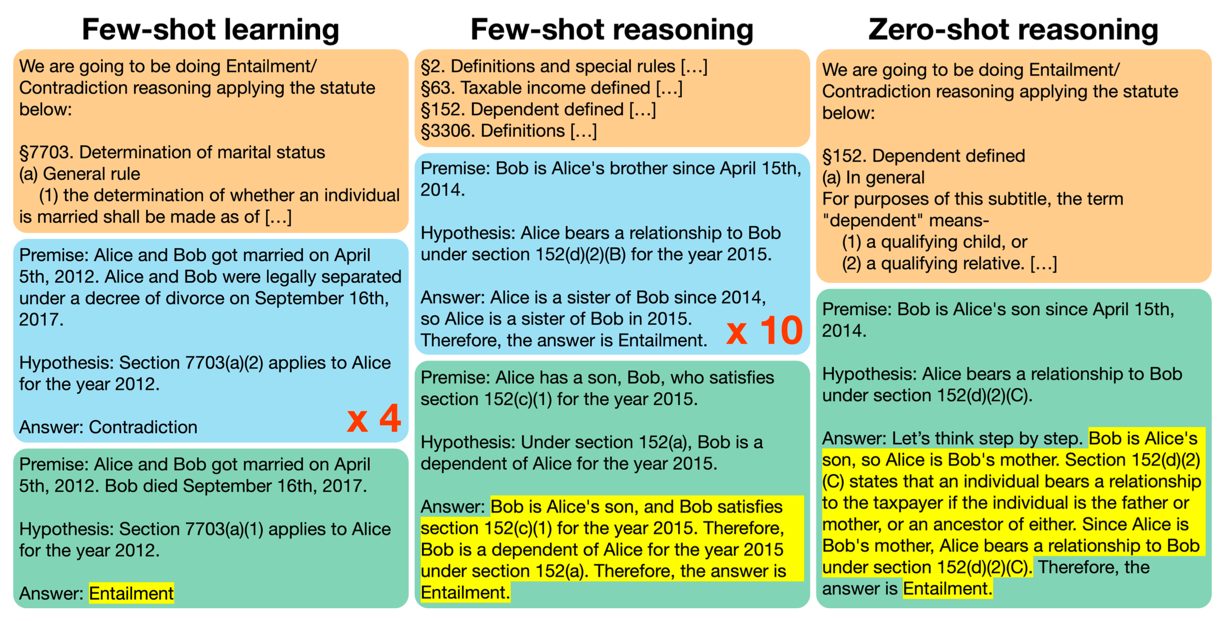
\includegraphics[width=\textwidth]{statutory}
	\caption{Prompts used in \textcite{blairstanek2023gpt3statutory} to pose SARA test cases to GPT-3. The top boxes, in orange, contain statutes (optional). Example cases are in blue; in zero-shot, no example cases exist. At the bottom, in green, are test cases. The text highlighted in yellow is generated by GPT-3. If GPT-3’s first response is unclear, the second prompt with "Therefore the answer is" is used, following \textcite{kojima2023large}. Source: \textcite{trautmann2022legalprompt}.}
	\label{fig:legal_prompting}
\end{figure}


\textcite{blairstanek2023gpt3statutory} evaluates the capacity of OpenAI's GPT-3 model, specifically text-davinci-003, to perform statutory reasoning\footnote{Statutory reasoning is the application of legal rules written by legislative bodies to facts that are also in natural language}, a fundamental skill in legal practice, on an established dataset known as SARA (StAtutory Reasoning Assessment).
The investigation includes several approaches like dynamic few-shot prompting, chain-of-thought prompting, and zero-shot prompting (examples in Figure~\ref{fig:legal_prompting}).

The model surpasses previous benchmarks yet still exhibits considerable room for improvement, especially when handling simple synthetic statutes, revealing limitations in its current statutory reasoning capabilities even though GPT-3 has some prior knowledge of the U.S.\ Code.

\begin{table}[!h]
	\centering
	\begin{tabularx}{\textwidth}{Xcccc}
		\toprule
		Method     & Constitutional Law & Taxation & Torts & Total \\
		\midrule
		Simple     & 21/25              & 24/60    & 6/10  & 51/95 \\
		CoT        & 21/25              & 18/60    & 5/10  & 44/95 \\
		Rank Order & 20/25              & 21/60    & 6/10  & 47/95 \\
		\bottomrule
	\end{tabularx}
	\caption{Comparison of Multiple Choice Methods. Source: \textcite{choi2023chatgptlaw}.}
	\label{tab:mc_comparison}
\end{table}

\textcite{choi2023chatgptlaw} explored ChatGPT's ability to write law school exams at the University of Minnesota Law School, encompassing multiple choice and essay questions across four courses.
ChatGPT generated answers for Constitutional Law, Employee Benefits, Taxation, and Torts exams, with varying question formats across these subjects.
These answers were blindly graded in line with the standard grading process.
ChatGPT managed to pass all four classes, averaging a C+ grade, demonstrating better performance on essay questions compared to multiple-choice, with notable strengths in organizing and composing essays (Table~\ref{tab:mc_comparison}).

Despite its overall passing performance, ChatGPT ranked at or near the bottom in each class.
The model's essays showcased a strong grasp of basic legal rules but struggled with issue spotting and detailed application of rules to facts.
The findings suggest that while ChatGPT can assist in legal education and potentially in legal practice, it currently lacks the nuanced understanding and depth of reasoning required for high-level legal analysis.

Recent studies on the latest GPT-4 model have shown that it can achieve a top 10\% score in a simulated bar exam compared with human test-takers~\cite{openai2024gpt4}, while \textcite{nay2022lawinformscode} and exhibit powerful abilities of legal interpretation and reasoning.
To further improve the performance of LLMs in the law domain, specially designed legal prompt engineering is employed to yield advanced performance in long legal document comprehension and complex legal reasoning~\cite{survey}.


\subsection{LLMs in Scientific Research}
\label{subsec:llms-in-scientific-research}

LLMs in scientific research can be employed across various stages of the research process, from literature review to hypothesis generation, brainstorming, data analysis, manuscript drafting, proofreading, and peer review.
Empirical evidence underscores the aptitude of LLMs in managing tasks dense with scientific knowledge, such as those presented by PubMedQA~\cite{jin2019pubmedqa} and BioASQ~\cite{krithara2022bioasq}.
It is particularly true for LLMs pre-trained on scientific corpora, including, but not limited to, Galactica~\cite{taylor2022galactica} and Minerva~\cite{lewkowycz2022minerva}.

Due to their capabilities, LLMs are poised to play an integral role as supportive tools throughout the scientific research process~\cite{zhang2023smallstep}.
During the initial stages of research, such as brainstorming, LLMs can assist in generating novel research ideas and hypotheses, thereby fostering creativity and innovation\footnote{Randomness and creativity of a model can be tuned using specific parameters. For example temperature is a OpenAI ChatGPT, GPT-3 and GPT-4 models parameter that govern the randomness and thus the creativity of the responses.}.

In the literature review phase, LLMs can perform exhaustive reviews, encapsulating the state of advancement within specific scientific disciplines~\cite{haman2023usingchatgpt, aydin2022openaichatgpt} providing explanations for scientific texts and mathematics with follow-up questions.

Progressing to the phase of research ideation, LLMs have displayed potential in formulating compelling scientific hypotheses~\cite{park2023chatgpt}.
In \textcite{park2023chatgpt}, the authors shows the ability of GPT-4 to generate hypotheses in the field of materials science, showcasing the model's capacity to propose research directions.
Through examining conversations, it was evident that GPT-4 generates richer and more specific information than the prompts provided, disproving the mirroring hypothesis.
While checking for verbatim copying was more challenging, GPT-4 does seem to reflect current academic trends to an uncanny degree.
However, it also combines disciplines and innovates concepts, leading to both errors and genuine creative insights.
The authors compared the process to how cosmic rays can drive biological evolution through mutations: radiations break DNA strands and cause cancer and deaths, but can also drive mutations and evolution of the biosphere.
Given the highlighted limitation, LLMs can be used to generate hypotheses for further human evaluation and refinement.

In the subsequent data analysis stage, LLMs can be harnessed for automating the examination of data attributes, including exploratory data analysis, visualization, and the extraction of analytical inferences~\cite{cheng2023gpt4dataanalyst}.
In \textcite{hassan2023chatgptdatascientist}, the authors demonstrate the utility of GPT-4 in automating data analysis tasks, such as data cleaning, feature engineering, and model selection, thereby streamlining the data science workflow.

Regarding proofreading, LLMs can enhance the quality of scientific manuscripts by identifying grammatical errors, improving readability, and ensuring adherence to academic conventions.
In addition, LLMs can go beyond helping users check grammar and can further generate reports about document statistics, vocabulary statistics, etc, change the language of a piece to make it suitable for people of any age, and even adapt it into a story~\cite{kim2022replacegrammarly}.
While ChatGPT has some usability issues when it comes to proofreading, such as being over 10 times slower than DeepL and lacking in the ability to highlight suggestions or provide alternative options for specific words or phrases~\cite{maximov2023englishgrammar}, it should be noted that grammar-checking is just the tip of the iceberg.
ChatGPT can also be valuable in improving language, text restructuring, and other writing aspects.

Furthermore, in the manuscript drafting phase, the utility of LLMs extends to aiding scientific writing endeavors~\cite{alkaissi2023artificialhallucinations, azaria2023chatgptexperts}, offering a multitude of services such as condensing existing materials and refining the written prose~\cite{buruk2023academicwriting}.
As explained in \textcite{buruk2023academicwriting} and \textcite{alkaissi2023artificialhallucinations}, LLMs can assist in generating abstracts, introductions, and conclusions, thereby enhancing the overall quality of scientific manuscripts.

Finally, in the peer review process, LLMs can contribute to automating the peer review process, undertaking tasks like error identification, compliance with checklists, and prioritization of submissions~\cite{liu2023reviewergpt}.

LLMs' utility spans beyond the aforementioned domains, with their deployment also being explored in the psychological sphere.
Here, studies have probed LLMs for human-like traits, encompassing self-perception, Theory of Mind (ToM)\footnote{The ability to impute unobservable mental states to others}, and emotional cognition~\cite{kosinski2023theoryofmind, amin2023affectivecomputing}.
\textcite{kosinski2023theoryofmind} employs classic false-belief tasks\footnote{A false-belief task is a psychological test used to assess an individual's ability to understand that others can have beliefs about the world that are different from their own and that these beliefs can be incorrect. This ability is a crucial component of the Theory of Mind (ToM), which is the capacity to attribute mental states—beliefs, intents, desires, emotions, knowledge, etc.—to oneself and others and to understand that others have beliefs, desires, and intentions that are different from one's own.

	The classic example of a false-belief task is the Sally-Anne test, used primarily with children. The test involves two dolls, Sally and Anne. Sally has a basket, while Anne has a box. In the presence of Sally, a marble is placed in Sally's basket. Sally then leaves the room, and while she's away, Anne takes the marble from Sally's basket and puts it in her box. The child is then asked where Sally will look for the marble when she returns. The correct answer is Sally's basket, where she left the marble. A child who can correctly predict where Sally will look for the marble demonstrates an understanding that Sally holds a false belief about the location of the marble.
	Successfully completing a false-belief task indicates that the individual can understand that others can hold false beliefs and that these beliefs can influence their actions, a critical step in the development of social cognition and empathy.}, revealing a marked improvement in ToM capabilities in more recent versions of GPT-3.
Specifically, the davinci-002 version solved 70\% of ToM tasks, while the davinci-003 version achieved a 93\% success rate, demonstrating performances akin to seven and nine-year-old children, respectively.
Notably, GPT-3.5's performance in ToM assessments parallels that of nine-year-olds, suggesting nascent ToM capabilities in LLMs.
The study hypothesizes that ToM-like abilities might emerge spontaneously in AI without explicit programming, especially in LLMs trained in human language.
In the context of AI, particularly in LLMs like GPT-3, the ability to perform well on false-belief tasks suggests a sophisticated level of language understanding and a rudimentary form of Theory of Mind, albeit not conscious or sentient like in humans.

Moreover, the application of LLMs in software engineering is also gaining traction, with initiatives in code suggestions~\cite{sridhara2023chatgptsoftware}, code summarizations~\cite{sun2023code}, and automated program repairs~\cite{xia2023conversationalrepair}.